\chapter{\label{app5:tournamentSurvey}Appendix}












\section{\label{app5:method}Method}



\subsection{\label{app5:procedure}Procedure}


\subsubsection{\label{app5:studyIntro}Study Introduction Script}

\begin{CJK}{UTF8}{gbsn}
  \begin{quotation}
    大家好,我是前澳大利亚国家队队员,现牛津大学博士生李杰。我在做一个调查,是关于橄榄球运动员在高水平比赛前后的感受。这项研究可能有助于提升职业橄榄球运动员在高水平比赛中的表现。请所有参加河北比赛的球员完成以下的调查。
    需要大约15分钟的时间完成。您所回答的问题对于我调查信息的准确性是十分重要的,所以请如实填写问卷。调查中的所有信息仅供研究使用,并对信息进行保密。有什么关于调查的问题请直接和我联系。感谢配合! 调查链接:
  \end{quotation}
\end{CJK}
%\url{<https://oxfordanthropology.qualtrics.com/SE/?SID=SV_7ZKXiVERWNLAKxf&Q_Language=ZH-S>}{<Qualtrics Survey>}}

\begin{quotation}
      \textit{``Hello everyone, I am former Australian 7s Representative and current Oxford University PhD candidate, Jacob Taylor (Li Jie). I am conducting a study about the experience of professional rugby players before, during and after high-level rugby competition. I hope that this research will contribute to an understanding of high-level athletic performance. Can every athlete participating in the Qianan National Tournament please complete the following survey. The survey will take about 15 minutes to complete. It is very important for the quality of the research that you answer questions honestly according to your own experiences. Survey responses are confidential and will be used for research purposes only. If you have any questions please get in touch with me. Thanks for your cooperation! Here is the survey link:''}
\end{quotation}










  \subsection{\label{app5:surveyItems}Survey Items}

  \begin{enumerate}
  \item Individual and team \textbf{performance}.
  \item Overall feeling of team coordination, or \textbf{``team click''}
  \item Feelings of \textbf{social bonding} within the team
  \item \textbf{Technical competence}.
  \item \textbf{Exertion}, \textbf{fatigue}, and \textbf{injury}
  \item \textbf{Personality} (ten-item personality measure (TIPI) questionnaire  \citep{Gosling2003})
  \end{enumerate}


    \subsubsection{\label{app5:surveyPre}Pre-Tournament Survey Items}


\myparagraph{\label{app5:performancePre}}

Five components of individual performance were included:
\begin{description}
\item[Passing Technique] - ``How do you feel about your passing technique over the past month?''
\item[Support Play In Attack] - ``How do you feel about your support play in attack over the past month?''
\item[1on1 Defence] - ``How do you feel about your 1on1 defence over the past month?''
\item[Effectiveness In Contact] - ``How do you feel about your effectiveness in contact over the past month?''
\item[Decision Making In Game-Play] - ``How do you feel about your decision making in game-play over the past month?''
Athletes responded to each item by moving a toggle left or right from its default centre position on a continuous 100-point scale (0 = ``Extremely bad'', 100 = ``Extremely good'').
\end{description}

Four components of team performance were included:
\begin{description}
\item[Coordination Of Defensive Line] - ``How do you feel about your team's coordination of the defensive line over the past month?''
\item[Coordination Of Attacking Line] - ``How do you feel about your team's coordination of the attacking line over the past month?''
\item[Support Play] - ``How do you feel about your team's support play over the past month?''
\item[On-field Communication] - ``How do you feel about your team's on-field communication over the past month?''
Athletes responded to each item by moving a toggle left or right from its default centre position on a continuous 100-point scale (0 = ``Extremely bad'', 100 = ``Extremely good'').
\end{description}

\begin{description}
\item[Performance On Mood] ``To what extent does the way you perform influence your mood?''
\item [Performance Confidence Future] ``To what extent does your recent performance influence your confidence for future performance?''
Athletes responded to each item by moving a toggle left or right from its default centre position on a continuous 100-point scale (0 = ``Not at all'', 100 = ``Extremely'').
\end{description}



\myparagraph{\label{app5:clickPre}Team Click}
The following items designed to measure ``team click'' were included in the pre-Tournament survey:
\begin{description}
  \item [Unspoken Understanding:] ``In the past month, how strong has the unspoken understanding been between team members?''  ``Unspoken understanding'' is an English translation of a Chinese term \textit{moqi}, which is often used in team sport contexts to express the idea of  ``group flow'' or ``team click.''
  \item [General Atmosphere:] ``How is the general atmosphere in the team in the past month?'' This question utilised the Chinese word \textit{qichang}, a term taken from Chinese qigong, literally meaning ``field of energy''. Qichang is commonly used to describe the atmosphere generated when the team is performing playing well.
  \item [Reliability Of Others:] ``During the past month, to what extent have you felt that you can rely on others to perform their roles on the field (for example, in key moments of competition or training)?'' - This item was designed to measure perceived reliability of teammates to successfully coordinate  on-field behaviour
  \item [Reliability For Others:] ``During the past month, to what extent have you felt that others can rely on you to perform your role on the field (for example, in key moments of competition or training)?'' Designed to measure the perception of the surveyed athlete's own reliability to perform on-field coordination tasks for other teammates:
  \item[Ability Extended By Others:] ``When coordinating with others on the field in the past month, do you feel that your individual ability is extended by the ability of your team mates?'' Designed to measure the extent to which the athlete feels that his or her ability is extended or enhanced by the ability of teammates.
  \item [Click Pictorial:] a novel visual item with five responses, ranging from less to more coordinated arrangements of dots (representing 12 athletes in the team). See Figure ~\ref{fig:clickPictorial}.
\end{description}

    \begin{figure}[htbp]
      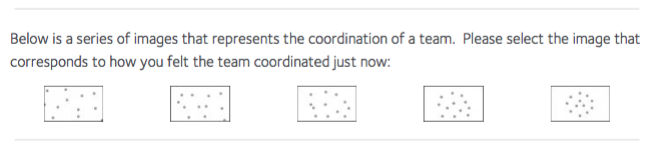
\includegraphics[width = \linewidth]{images/teamClickPictorial.png}
      \caption{Click Pictorial Scale}
      \label{fig:clickPictorial}
    \end{figure}


\myparagraph{\label{app5:bondingPre}Social Bonding}

  \begin{description}
    \item [Emotional Support] ``How emotionally supportive does the team feel?''
    \item [Shared Goal] ``How strong is the feeling that everyone is working towards a shared goal?''

    \item [Group Identification Verbal] A six-item scale designed to measure an individual's personal identification with the stereotypical features of the in-group  \citep{Mael1992}.  All 6 items were measured using a 5-point Likert scale.

  1. When someone critizes my team, it feels like a personal insult
  2. I am very interested in what others think about my team
  3. When I talk about my team, I usually say “we” rather than “they"
  4. This team's successes are my successes
  5. When someone praises my team, it feels like a personal compliment
  6. If a story in the media criticized my team, I would feel embarrassed

  \item [Identity Fusion Verbal] A seven-item scale designed to measure an individual's ``feeling of oneness with the group'' \citep{Swann2009}.  Identity Fusion is differentiated from Group Identification in its ability to account for an individual's felt, emotional and personal agentic associations with being a member of the target in-group \citep{Swann2012a}.  All 7 items were measured using a 5-point Likert scale.

  1. I am one with my team.
  2. I feel immersed in my team.
  3. I have a deep emotional bond with my team.
  4. My team is me.
  5. I’ll do for my team more than any of the other team members would do.
  6. I am strong because of my team.
  7. I make my team strong.

  \item [Identity Fusion Pictorial] A visual scale designed to measure Identity Fusion to the target in-group \citep{Swann2009}. The pictorial scale depicts two circles, one smaller circle to denote the individual, and one larger circle to denote the group, progressively moving closer to each other such that the most ``fused'' option depicts the smaller circle encased by the larger circle. The scale offers a total of five options to chose from, see Figure ~\ref{fig:fusionPictorialGroup}.  A total of three pictorial scales were included, each with different target in-groups: team, family, and country (China).

  \item [Fusion Pictorial Rank] Athletes were asked to rank their fusion to team, family, and country \citep{Whitehouse2014}.  ``Thinking about these relationships [to team, family, and country] please rank them below in order of which you feel most connected to. 1 for most connected, 3 for least connected.''
  \end{description}


  \begin{figure}[htbp]
    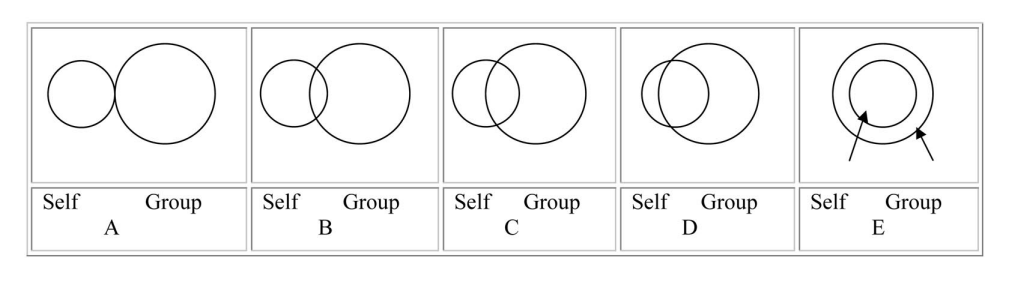
\includegraphics[width=\linewidth]{images/Identity_Fusion_Pictorial_Scale.png}
    \caption{Identity Fusion Pictorial Scale}
    \label{fig:fusionPictorialGroup}
  \end{figure}


\myparagraph{\label{app5:technicalCompetence}Subjective and Objective measures of technical competence}
Athletes were asked about their individual technical competence: ``Rate your individual ability in rugby, relative to: 1) Other teammates currently in your team, 2) Other current professional Chinese rugby players, 3) Professional rugby players form other countries.'' (Items were measured with a zero-centred 100 point scale, -50 - ``Extremely weak'', 0 - ``Average'', 50 - ``Extremely strong'').  Athletes were also asked about perceived competence of their team relative to other Chinese provincial teams: ``Rate your team's overall ability, relative to other teams in China'' (100 point scale, -50 - ``Extremely weak'', 0 - ``Average'', 50 - ``Extremely strong'').  In addition, athletes were asked if their perception of recent performance influences their 1) mood and 2) confidence regarding future performance (All these items were measured with a zero-centred 100 point scale, -50 - ``Extremely weak'', 0 - ``Average'', 50 - ``Extremely strong'').

Athletes were asked to report rugby-related attributes that would provide a more objective indicator of technical competence. These measures included: 1) rugby training age (number of years of experience training for rugby, to the nearest number of years), 2) the number of years spent training with the provincial teams (to the nearest year) , 5) whether the athlete is a usual member of the provincial program's starting team or the reserves.


\myparagraph{\label{app5:TIPI}Ten Item Personality Index}
Athletes were asked to indicate on a 7-point Likert scale the extent to which they agreed with 10 pairs of adjectives as appropriate descriptions of their personality. For example: ``I see myself as: dependable, self-disciplined'' (Response: 1 - ``Disagree strongly'', 2 - ``Disagree moderately'',  3 - ``Disagree a little'', 4 - ``Neither agree nor disagree'', 5 - ``Agree a little'', 6 - ``Agree moderately'', 7 - ``Agree strongly''). In the TIPI, two survey items corresponded to each of the big-five personality types, as follows:

\begin{description}
\item [Extraversion:] 1. Extraverted, enthusiastic; 6. Reserved, quiet (Reversed scale)
\item [Agreeableness:] 2. Critical, quarrelsome (Reversed); 7. Sympathetic, warm
\item [Conscientiousness:] 3. Dependable, self-disciplined; 8. Disorganised, careless (Reversed)
\item [Emotional Stability:] 4. Anxious, easily upset (Reversed); 9. Calm, emotionally stable.
\item [Openness to Experiences:] 5. Open to new experiences, complex; 10.Conventional, uncreative (Reversed)
\end{description}



\myparagraph{\label{app5:additionalPre}Additional Items}
Athletes were asked about their feelings regarding their team's commitment to aspects of team discipline over the past month (punctuality to training and team meetings, observing bed times and curfews, attendance at meals, general team conduct) (100 point scale for each item, 0 - ``Extremely poor'', 100 - ``Extremely strong'')).

NAME
DOB
PLAYING POSITION
INJURY










\subsubsection{\label{app5:surveyMid}Mid-Tournament Survey Items}



Athletes were asked to report on various components of physical and mental fatigue, exertion, and injury.

Following each mid-Tournament survey and in the post-Tournament survey, athletes were asked about their mood (``How are you feeling now after the tournament?'') and responded by choosing a point on a 10-point scale between three pairs of emotions (``Not aroused / highly aroused'',  ``Depressed/Relaxed'' and  ``Nervous/Excited'').\footnote{Many athletes experienced difficulty filling out this item in the survey, as such it was not included in the analysis} Athletes were also asked about feelings of fatigue ``How fatigued do you feel as a result of the game/tournament?'', perceived physical exertion (Borg RPE scale, \citep{Borg1990} and perceived mental exertion using two 15-point scales \citep[see][ ]{Noakes2012a}.  Athletes were also asked to indicate their injury status on a 100-point scale (0 = ``Unable to play'', 100 = ``Completely fit to play'').  A baseline measure of injury was  collected in the pre-Tournament survey, but fatigue, exertion, and mood measures were not included in the pre-Tournament survey because of inappropriateness for the pre-Tournament context.









\subsubsection{\label{app5:surveyPost}Post-Tournament Survey Items}






\subsubsection{\label{app5:objectivePerformance}Objective Performance Measures}

\begin{description}
\item [Final Rank:] A rank was given to each team based on performance in their respective competition (men's   women's). These rank scores were then reversed for the purposes of statistical analysis (1st place in men's Tournament (8 teams) = 8, 2nd place = 7, and so on)
\item [Total Wins - Losses:] A team's total number of losses was subtracted from its total number of wins.  Thus, more successful teams overall had a higher score.
\item [Total Minutes:] Total number of minutes played throughout the Tournament by each individual athlete
\item [Total Points:] Total number of points scored throughout the Tournament by each individual athlete
\item [Starting Team Average] An average measure indicating likelihood of an athlete being selected in the starting team. Each Athlete was awarded 1 point for each game he or she started in the starting team; reserve squad athletes were awarded zero for each game. Each athlete's total was divided by the total number of games that they participated in during the Tournament, including games in which they didn't take the field, to produce an average score for the Tournament.
\end{description}
























\section{\label{app5:stats}Statistical Method}

\subsection{\label{app5:EFA}Data Reduction using Exploratory Factor Analysis}
EFA is one of various available data reduction techniques, and is distinct from its main alternative, Principal Components Analysis (PCA), in that it is capable of modelling the latent dimensions of a collection of variables.\footnote{PCA is concerned only with establishing which components exist within the existing data and how a particular variable might contribute that component. To do this, PCA makes the assumption that all variance in a subset of variables is common variance, and therefore communality between all variables is equal to 1. From this assumption, the original data can be transposed into a linear model without the need for a communality-dependent estimated coefficient for each variable \citep{Widaman2007}. EFA examines all the pairwise relationships between individual variables and seeks to extract latent factors from the measured variables.  Squared Multiple Correlations (which are essentially multiple regressions in which each variable is predicted by all others) were used to calculate the common variance (communality) between each variable in an analysis (the communality value is much like an R-squared value from a multiple regression).
The square root of the communality score for each variable is then used as a coefficient that conditions the relationship between each variable and the underlying dimensions (factors) identifiable in the data. Also known as ``factor loadings,'' these coefficients become the parameters of linear model capable of estimating factor scores for each individual observation, which can be utilised in subsequent statistical analysis in place of single variable observations.

A final step in the EFA procedure is the process of ``rotation'', which is an optimisation technique designed to encourage each variable to load on as few factors as possible \citep{Rummel1988}. Rotation refers to a geometric conception of factor analysis, in which individual variables can be plotted in n-dimensional space according to their relationship to each dimension (factor). By rotating the axes of these dimensions, the distance of a given variable to that dimension can be reduced, which results in an increase in factor loading on one factor and (ideally) a decrease in factor loading on another uncorrelated variable. Orthogonal (or perpendicular) rotation of axes refers to axes, say X and Y, maintaining a 90-degree perpendicularity and rotating clockwise or anticlockwise, depending on the location of the variable clusters.
Orthogonal rotation thus enables optimisation of loadings for clusters of variables that are distant from each other in n-dimensional space. If correlation exists between clusters of variables, however, rotating axes obliquely (inwards towards each other) provides a more effective way of reducing the distance between clusters of variables and the latent dimensions that account for such clustering \citep{Osborne2015}. See Figure ~\ref{fig:orthogonalOblique} for a graphical  illustration of the difference between orthogonal and oblique rotation. Given that most variables of interest in the present study were correlated to some degree, I opted for an oblique rotation method \citep{Field2012}. EFAs were conducted using the factanal() function in the Stats package (Version 3.3.0) in R, using the ``promax'' (oblique) rotation method \citep{Gorsuch1983}. Factor scores were standardised z-scores: zero-centred, with a standard deviation of 1.

\begin{figure}[htbp]
  \begin{center}
    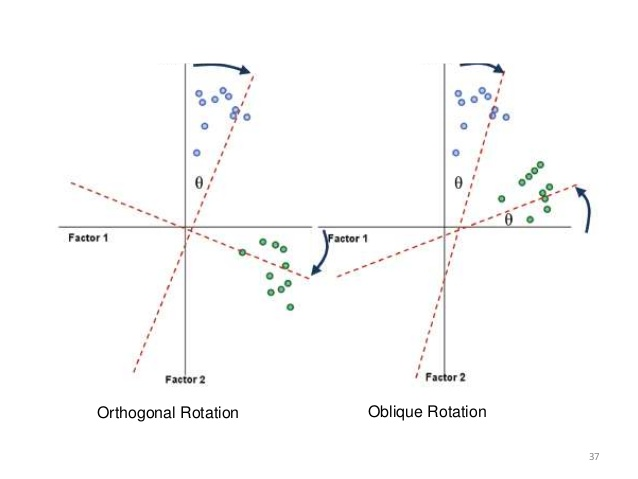
\includegraphics[width= \linewidth, scale = .5]{images/orthogonalObliqueRotationExample.jpg}
    \caption{Orthogonal and oblique rotation methods}
    \label{fig:orthogonalOblique}
  \end{center}
\end{figure}



\section{\label{app5:ICC}Intra Class Correlation}
For team-level variance, a one-way random effects model was used, in which average within-team variance (Mean Square Within) of the response variable was divided by the average total variance of the response (Mean Square Total) \citep{Field2005a}.  Each athlete is member of one of 15 teams, which are considered to be sampled from a larger pool of potential teams, hence treated as random effects. The ICC is then interpreted as the percentage of total variance accounted for by group-level variables \citep{Wolak2012}.
To statistically account for the unbalanced design of the data, an adjusted sample-size coefficient (k) was calculated using an equation provided by \citep{Lessells1987}.  While there is no firm agreement on what is deemed meaningful within-group variance, an ICC ratio of $>.10-1.00$ with confidence intervals that do not include zero was considered a strong indication of non-random correlation of group-level residuals \citep{Bailey2011}. As Table ~\ref{tab:ICCsummaryTeam} and ~\ref{tab:ICCsummarySex} indicate, small to moderate team-level intra-class correlation of responses exist for factors of Objective Competence, Joint Action Success, Individual Performance Success, and Team Click. ICCs for Social Bonding and Fatigue meanwhile were relatively low (all $r's <.1$). Sex-level ICCs were all relatively low, suggesting that sex-level variation could be ignored in subsequent inferential analyses.\\


































\section{\label{app5:results}Results}
\subsection{\label{app5:modelRobustness}Model Robustness Checks}


\begin{figure}[htbp]
    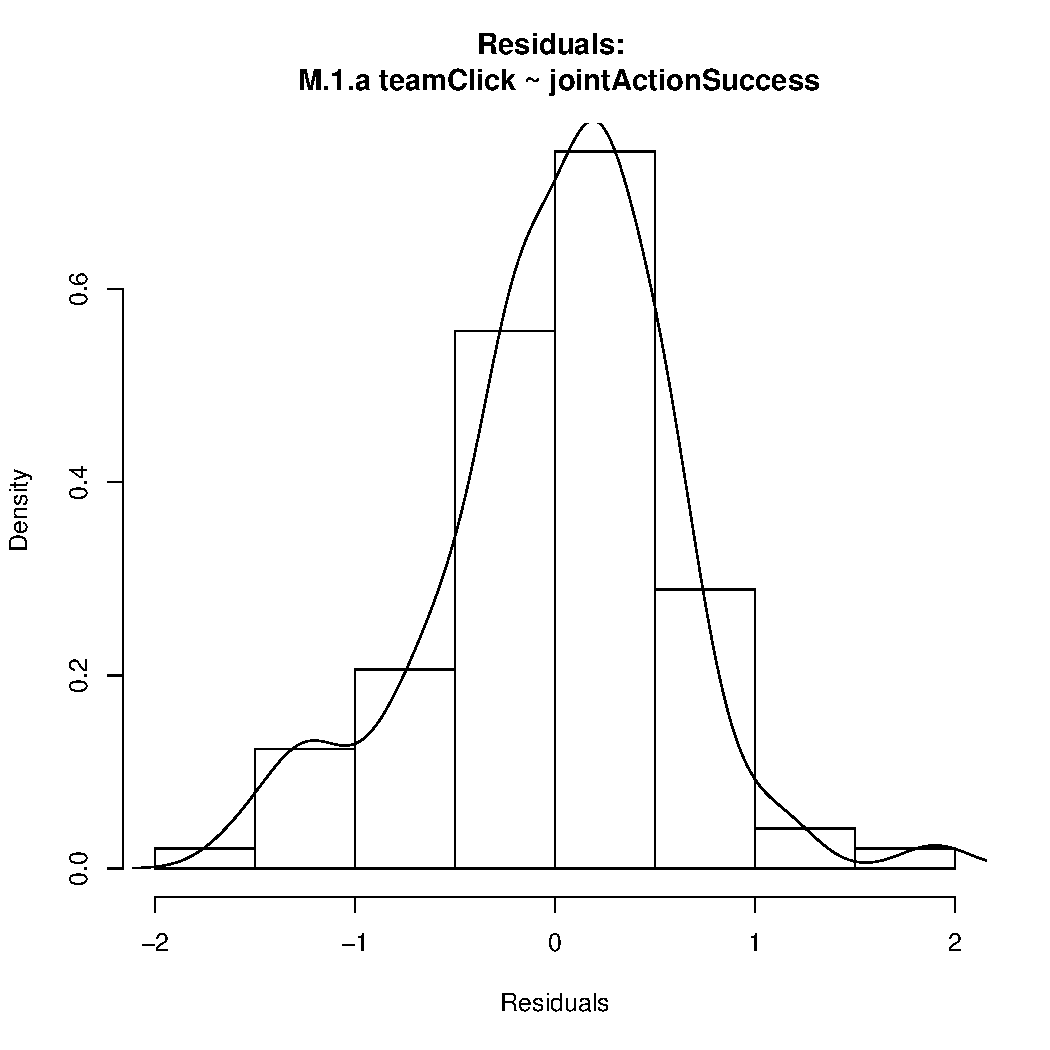
\includegraphics[scale =.4]{images/MLM1aHist.pdf}
    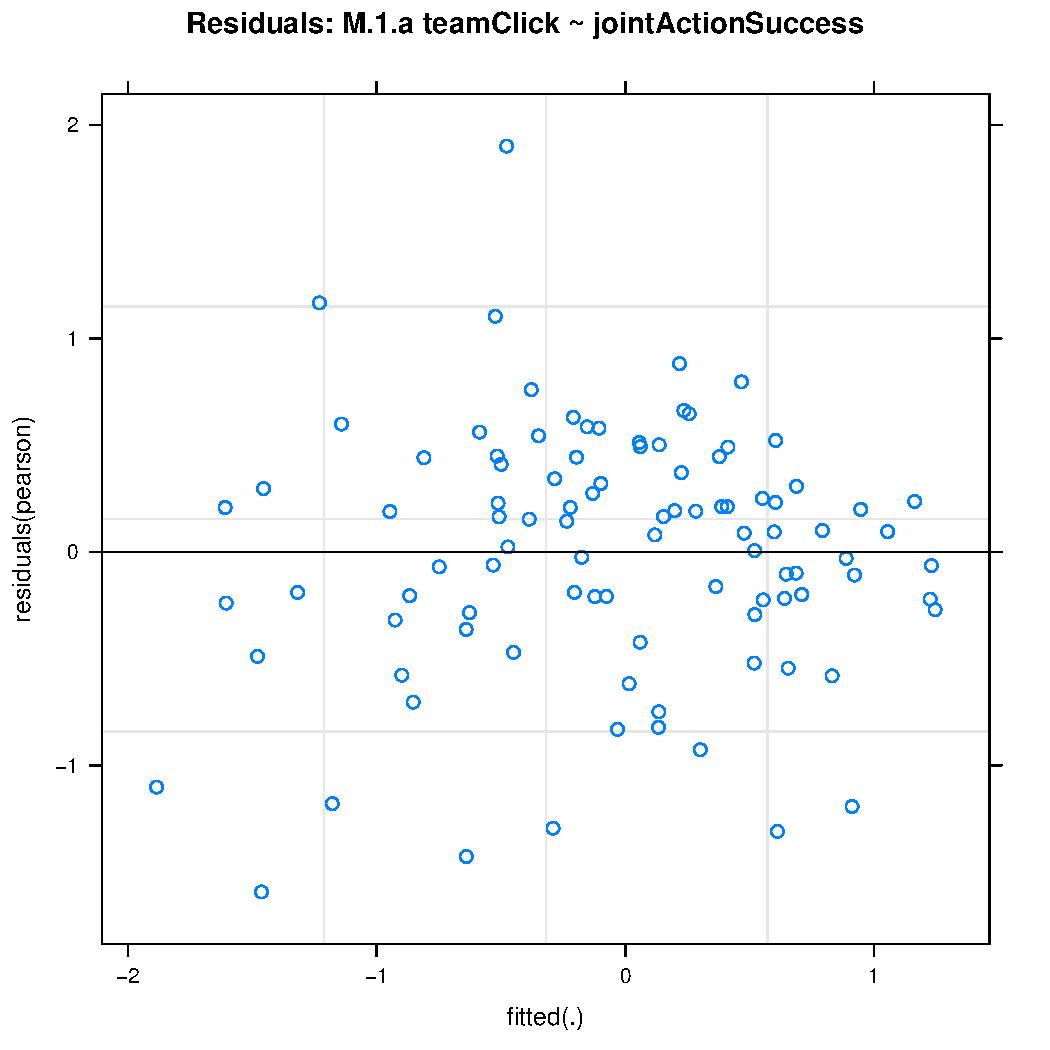
\includegraphics[scale =.4]{images/MLM1aScatter.pdf}
    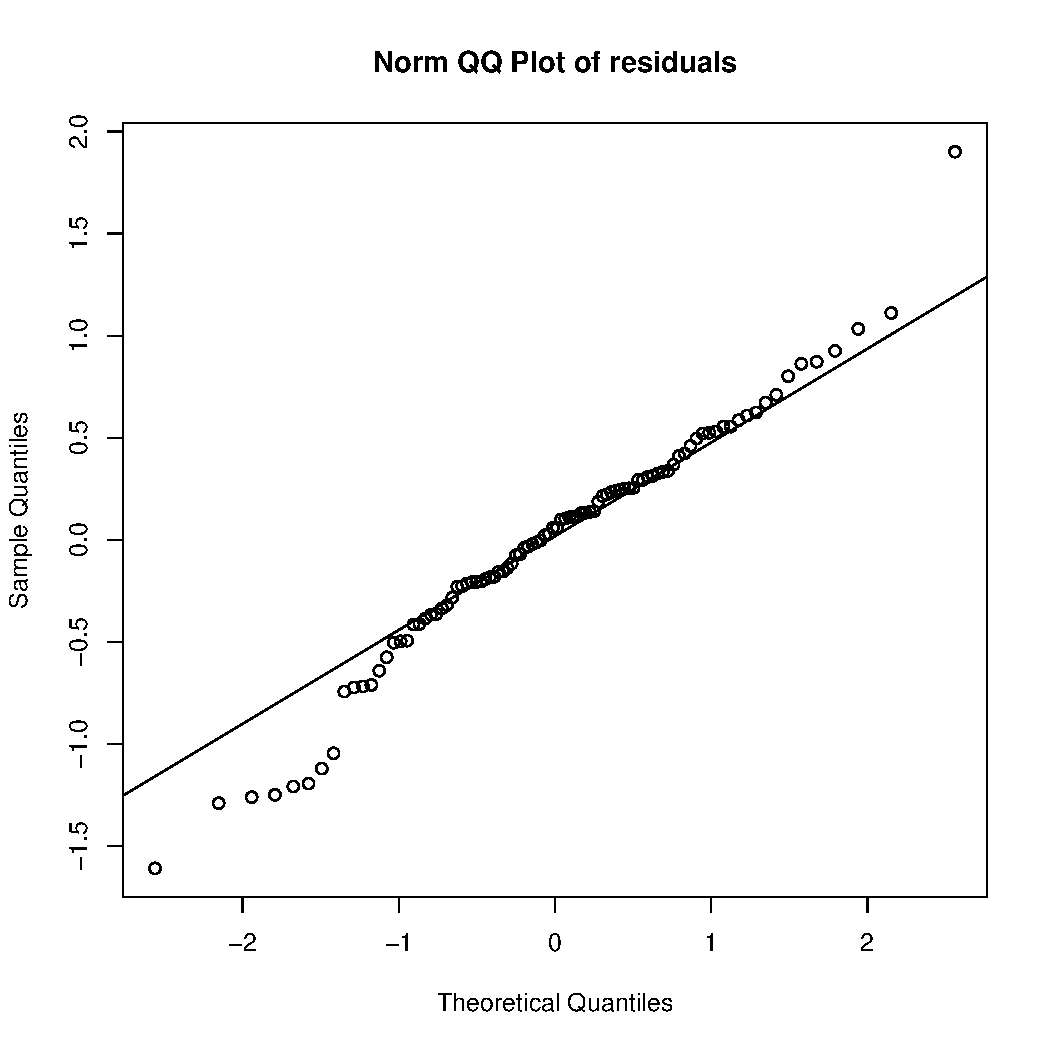
\includegraphics[scale =.4]{images/MLM1aQQPlot.pdf}
    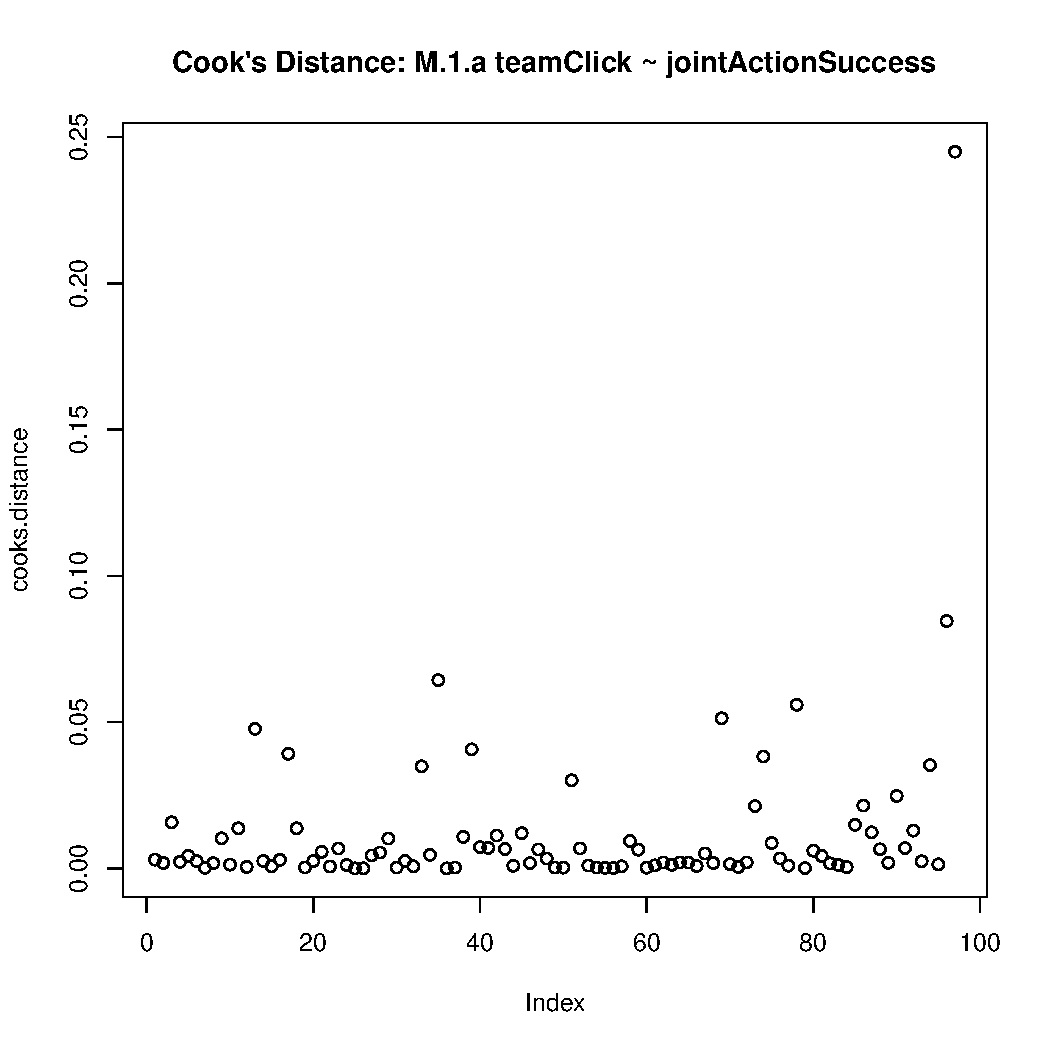
\includegraphics[scale =.4]{images/MLM1aCooksD.pdf}
    \caption{Model Assumptions: 1.a Joint Action Success Predicts Team Click}
    \label{fig:MLM1aAssumptions}
\end{figure}





\begin{figure}[htbp]
  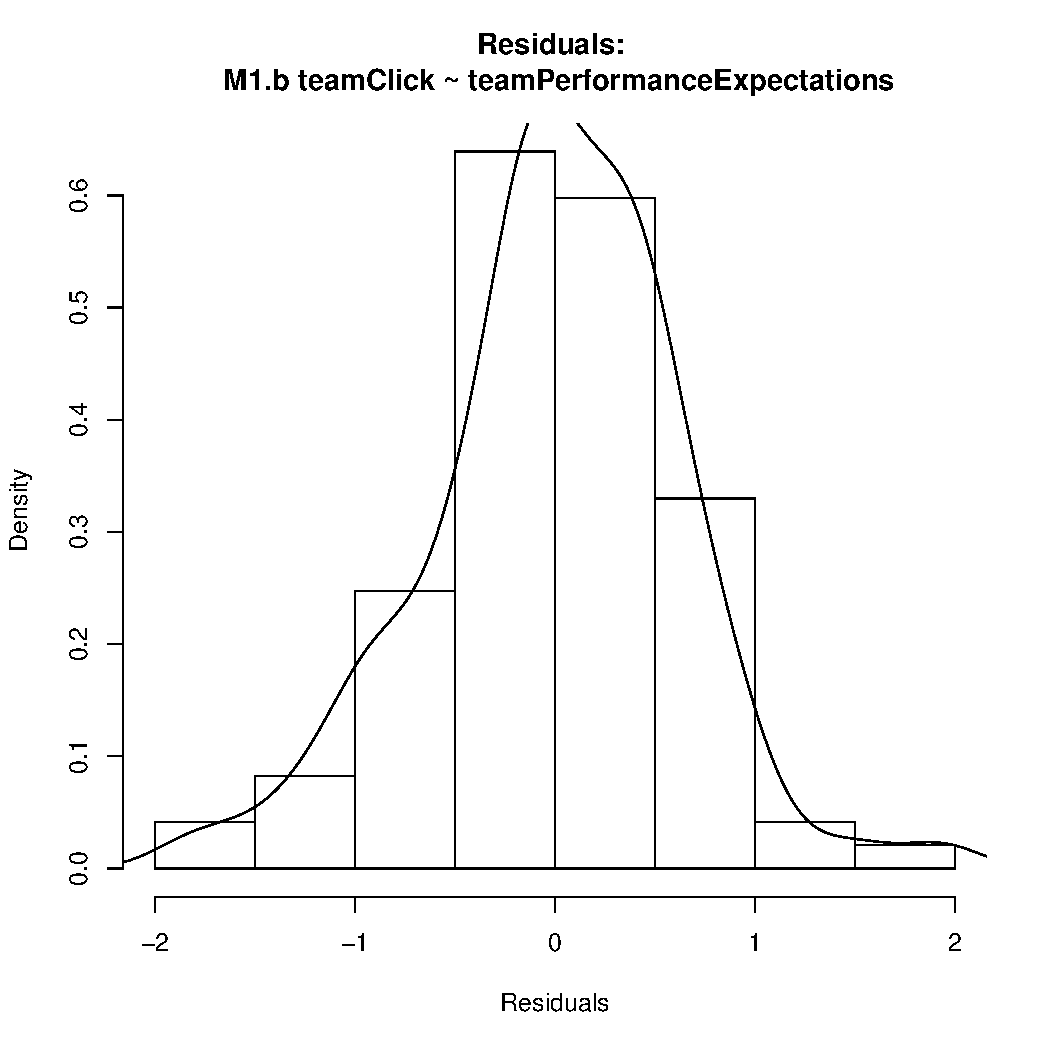
\includegraphics[scale =.4]{images/MLM1bHist.pdf}
  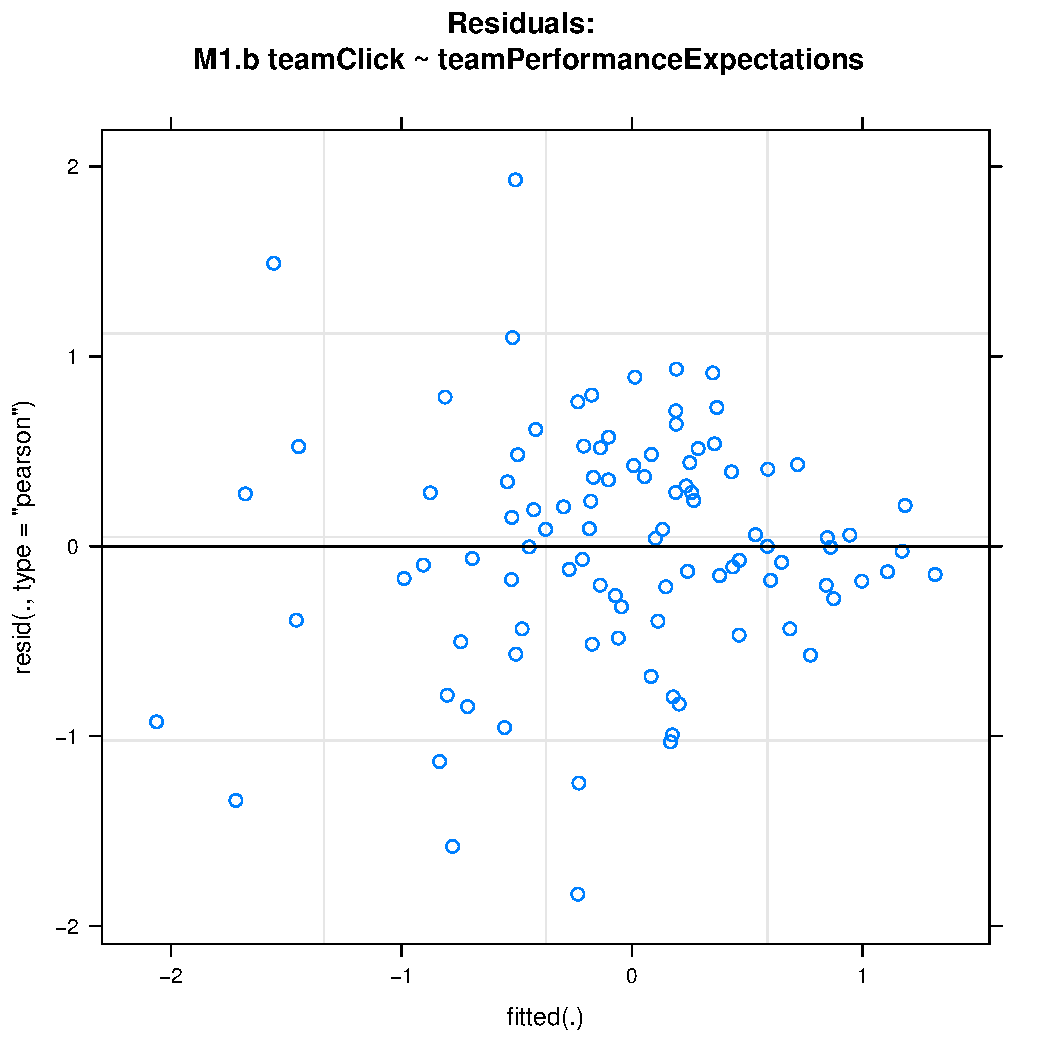
\includegraphics[scale =.4]{images/MLM1bScatter.pdf}
  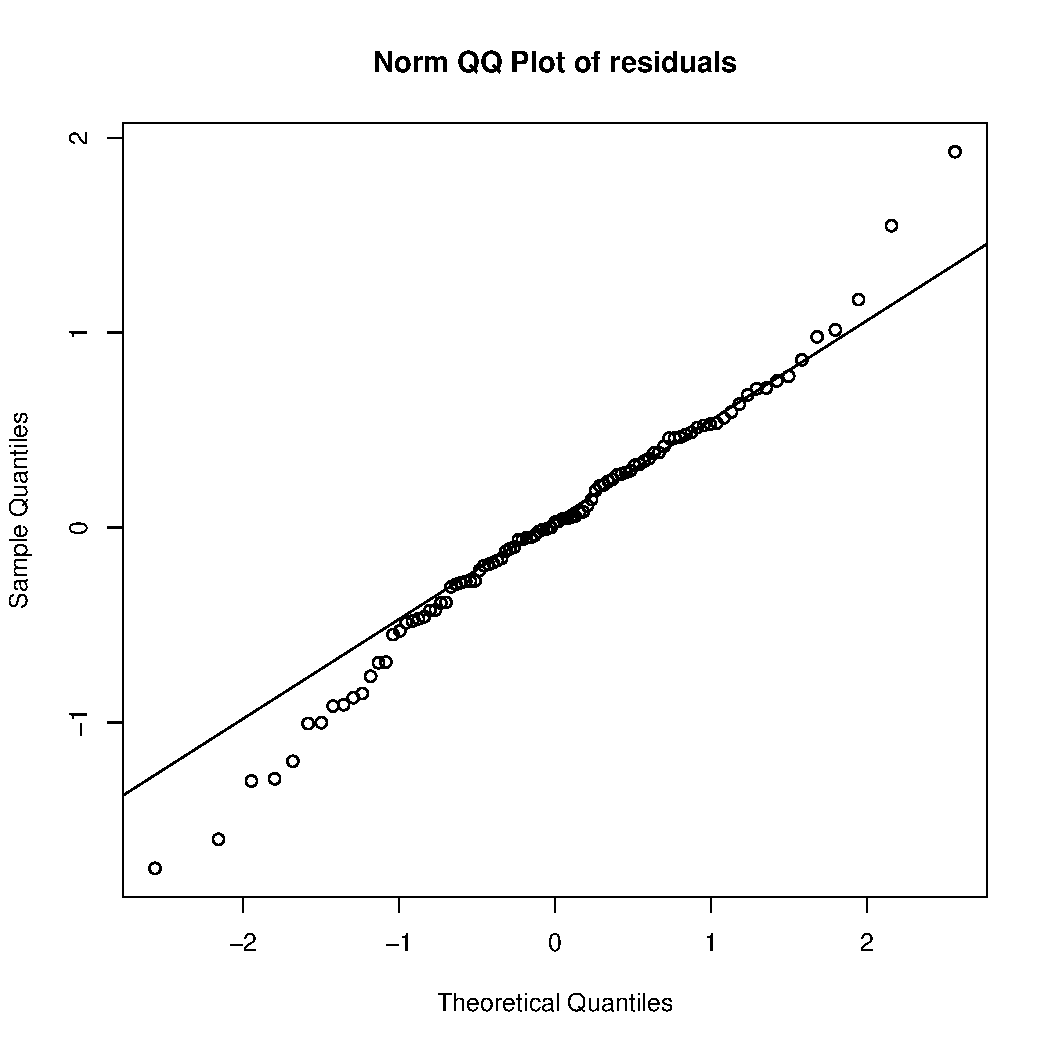
\includegraphics[scale =.4]{images/MLM1bQQNorm.pdf}
  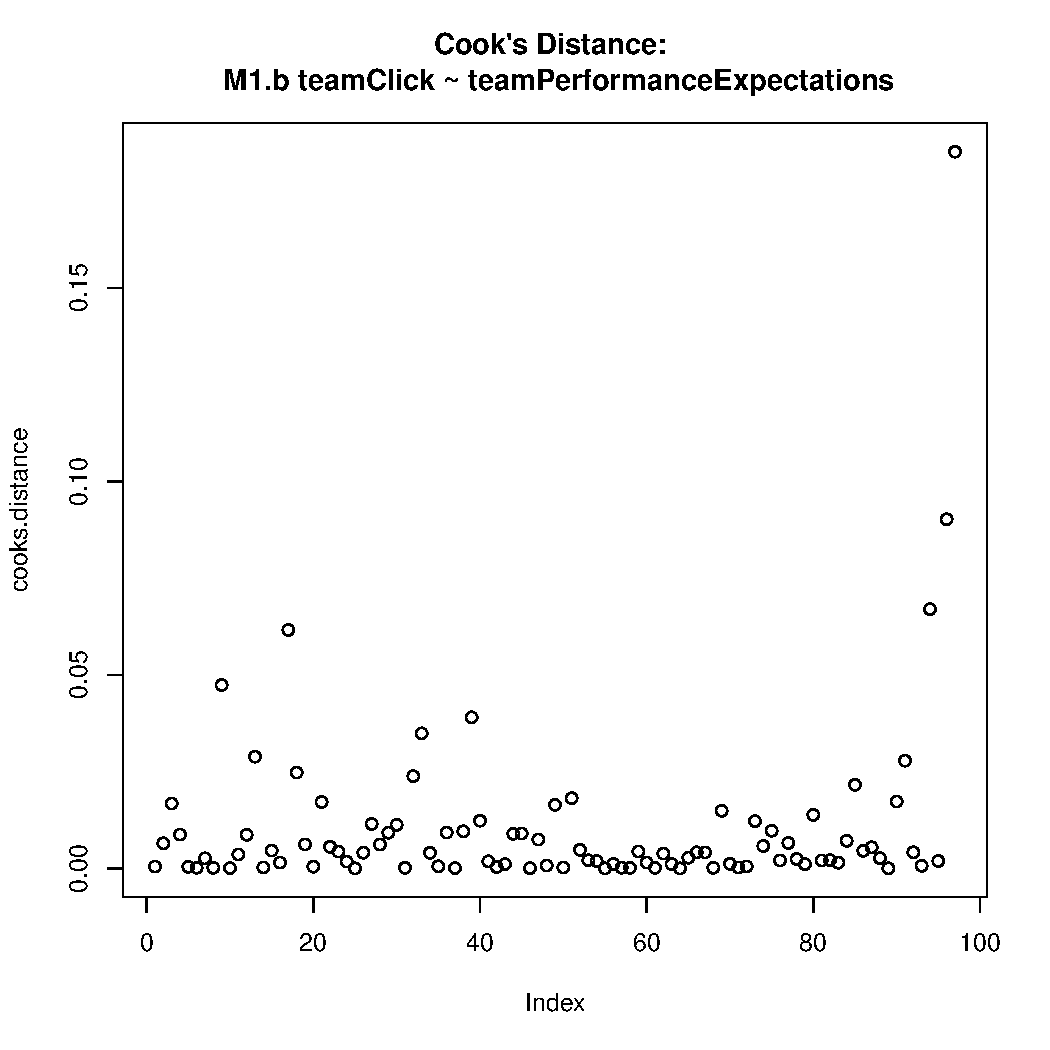
\includegraphics[scale =.4]{images/MLM1bCooksD.pdf}
  \caption{Model Assumptions: Model 1b Team Performance Expectations predict Team Click}
  \label{fig:MLM1bAssumptions}
\end{figure}





% Table created by stargazer v.5.2 by Marek Hlavac, Harvard University. E-mail: hlavac at fas.harvard.edu
% Date and time: Mon, Jun 26, 2017 - 20:35:23
\begin{table}[!htbp] \centering 
  \caption{teamClick = jointActionSuccess X teamPerformanceExpectations} 
  \label{tab:MLM1cPerformanceClickInteraction} 
\footnotesize 
\begin{tabular}{@{\extracolsep{5pt}}lc} 
\\[-1.8ex]\hline 
\hline \\[-1.8ex] 
 & \multicolumn{1}{c}{\textit{Dependent variable:}} \\ 
\cline{2-2} 
\\[-1.8ex] & teamClick \\ 
\hline \\[-1.8ex] 
 (constant) & $-$0.83$^{*}$ \\ 
  & (0.41) \\ 
  & \\ 
 jointActionSuccess & 0.57$^{*}$ \\ 
  & (0.25) \\ 
  & \\ 
 teamPerformanceExpectations & 0.01 \\ 
  & (0.005) \\ 
  & \\ 
 indPerformanceSuccess & 0.01 \\ 
  & (0.10) \\ 
  & \\ 
 indPerformanceExpectations & $-$0.001 \\ 
  & (0.003) \\ 
  & \\ 
 objectiveCompetence & 0.06 \\ 
  & (0.08) \\ 
  & \\ 
 subjectiveCompetence & 0.10 \\ 
  & (0.07) \\ 
  & \\ 
 finalRank & 0.03 \\ 
  & (0.04) \\ 
  & \\ 
 minutesTotal & 0.01 \\ 
  & (0.003) \\ 
  & \\ 
 pointsTotal & 0.004 \\ 
  & (0.01) \\ 
  & \\ 
 teamPerformanceComponentsFactorPost:teamPerformance7 & 0.0001 \\ 
  & (0.003) \\ 
  & \\ 
\hline \\[-1.8ex] 
Marginal R-squared & .56 \\ 
Conditional R-squared & .65 \\ 
Observations & 97 \\ 
Log Likelihood & $-$90.96 \\ 
Akaike Inf. Crit. & 217.91 \\ 
Bayesian Inf. Crit. & 264.26 \\ 
\hline 
\hline \\[-1.8ex] 
\textit{Note:}  & \multicolumn{1}{r}{$^{*}$p$<$0.05; $^{**}$p$<$0.01; $^{***}$p$<$0.001} \\ 
\end{tabular} 
\end{table} 






\begin{figure}[htbp]
  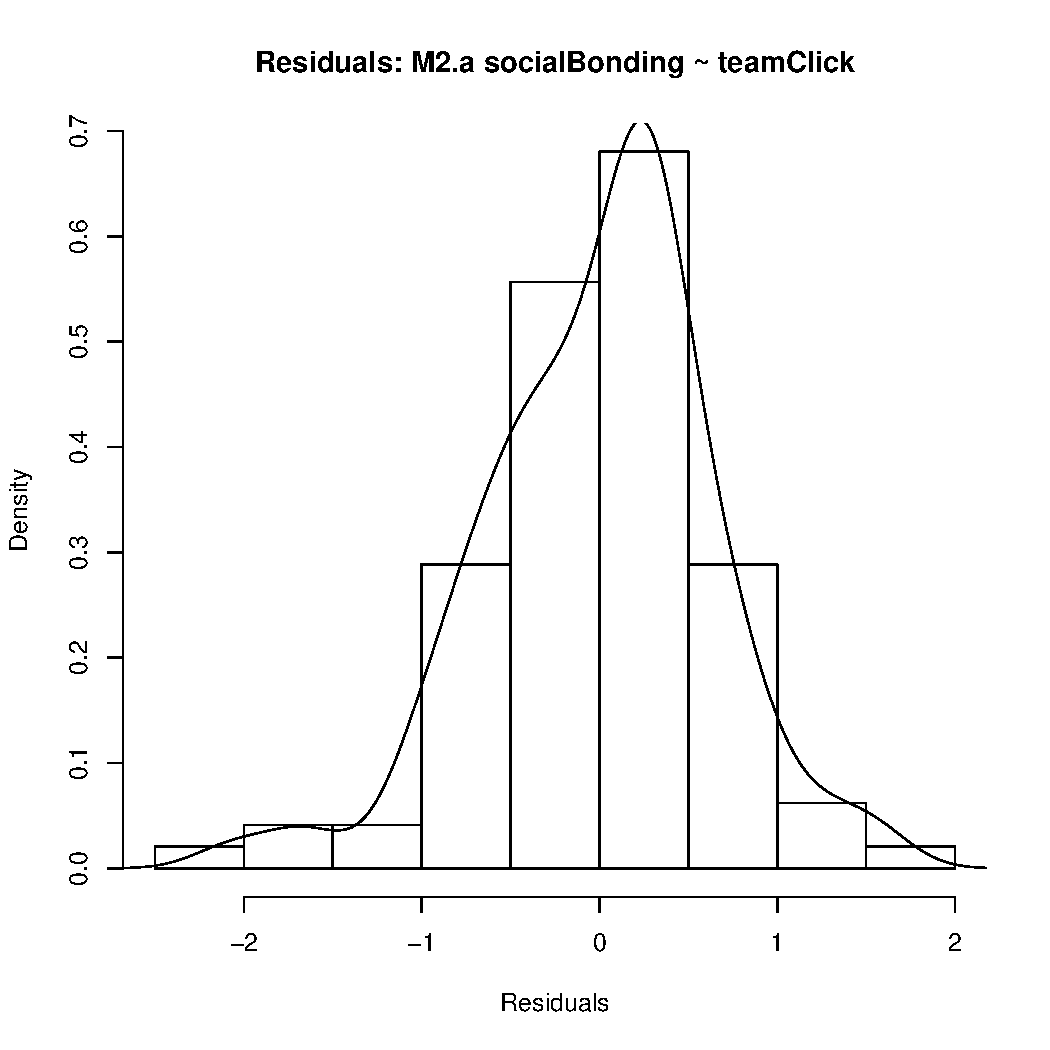
\includegraphics[scale =.4]{images/MLM2aHist.pdf}
  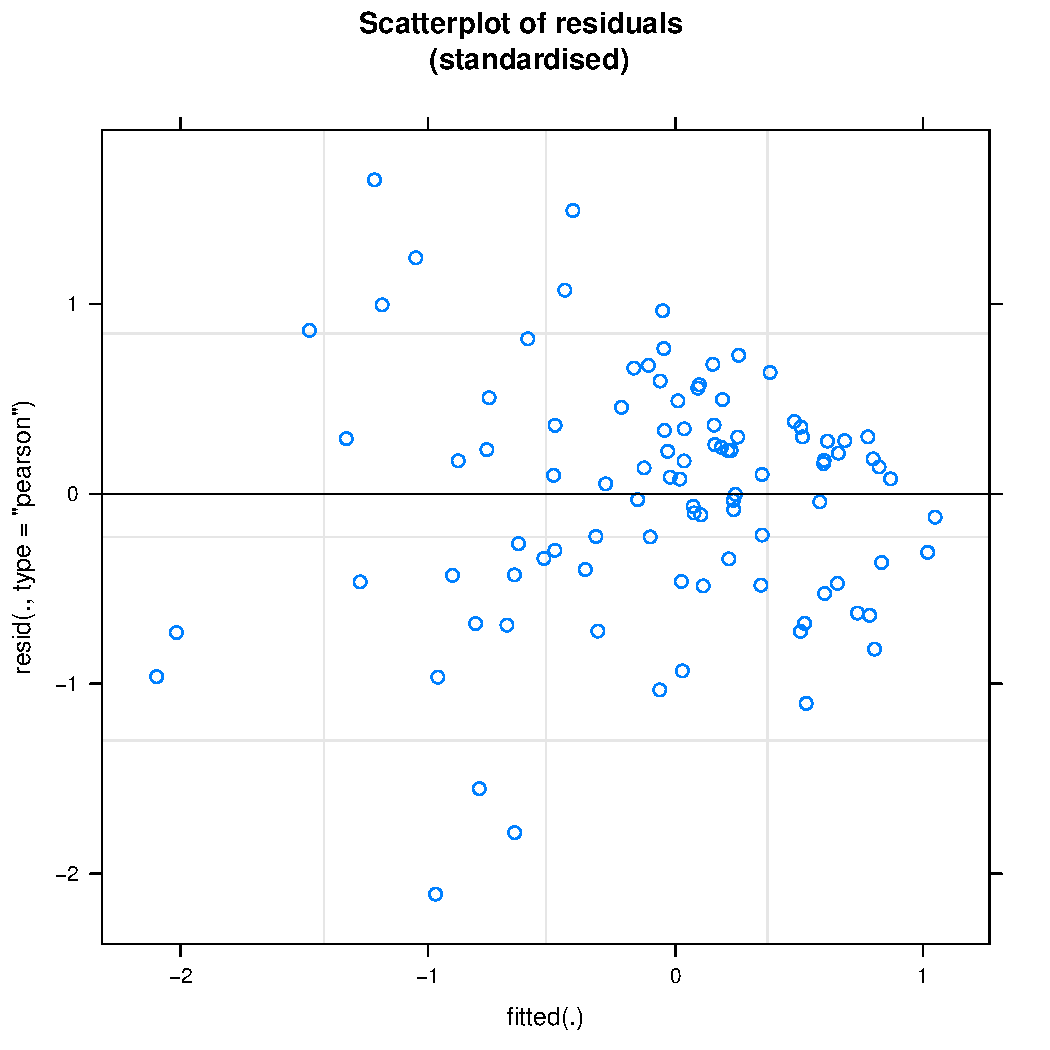
\includegraphics[scale =.4]{images/MLM2aScatter.pdf}
  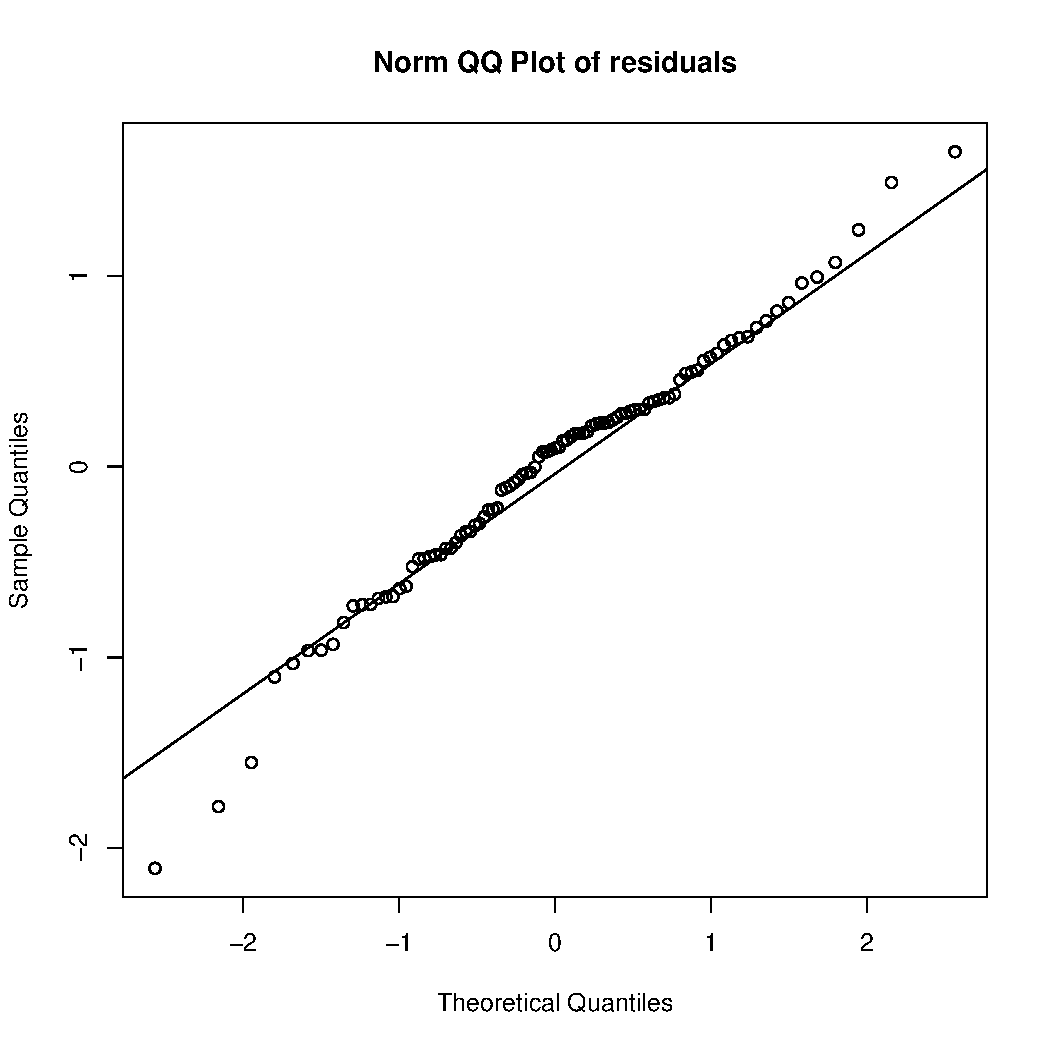
\includegraphics[scale =.4]{images/MLM2aQQNorm.pdf}
  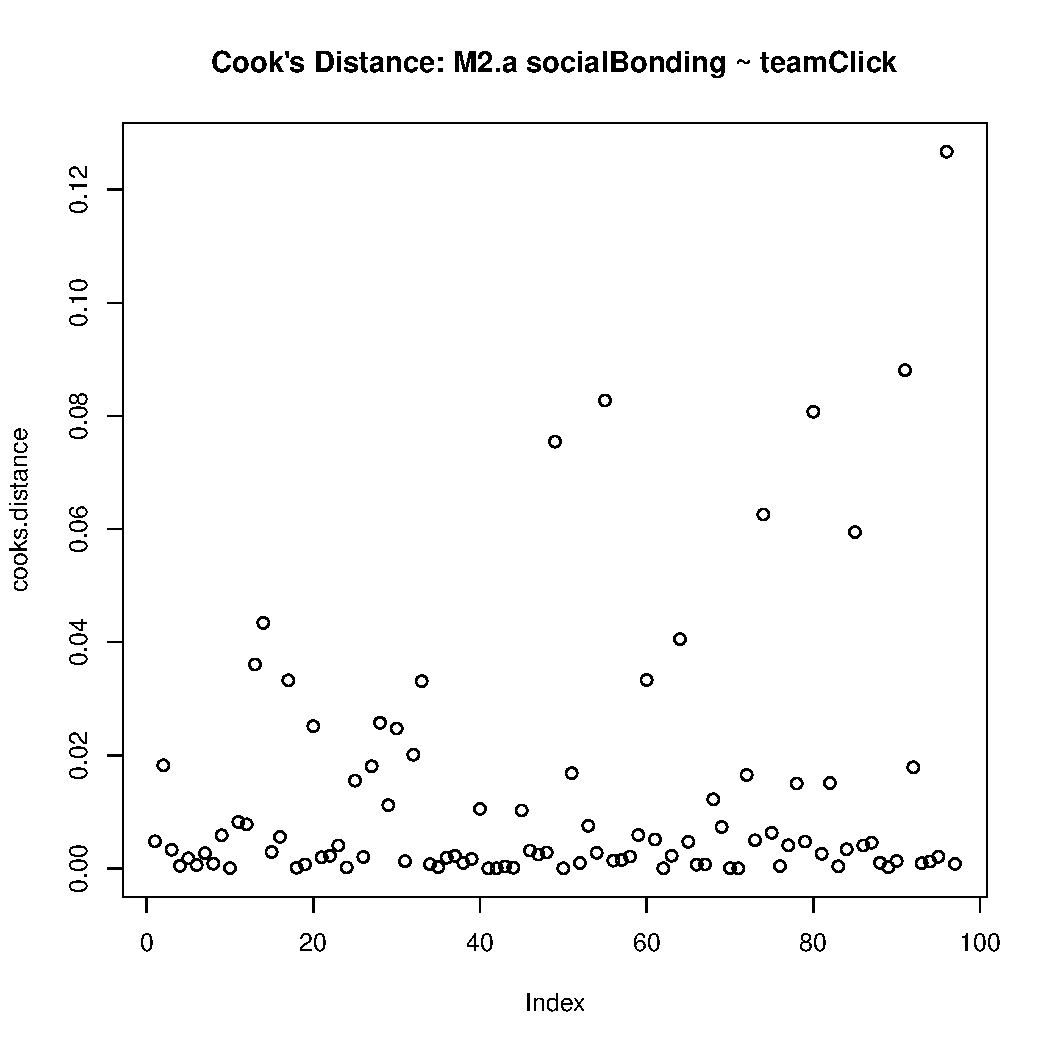
\includegraphics[scale =.4]{images/MLM2aCooksD.pdf}
  \caption{Model Assumptions: M2a Team Click predicts Social Bonding}
  \label{fig:MKM2aAssumptions}
\end{figure}





\begin{figure}[htbp]
  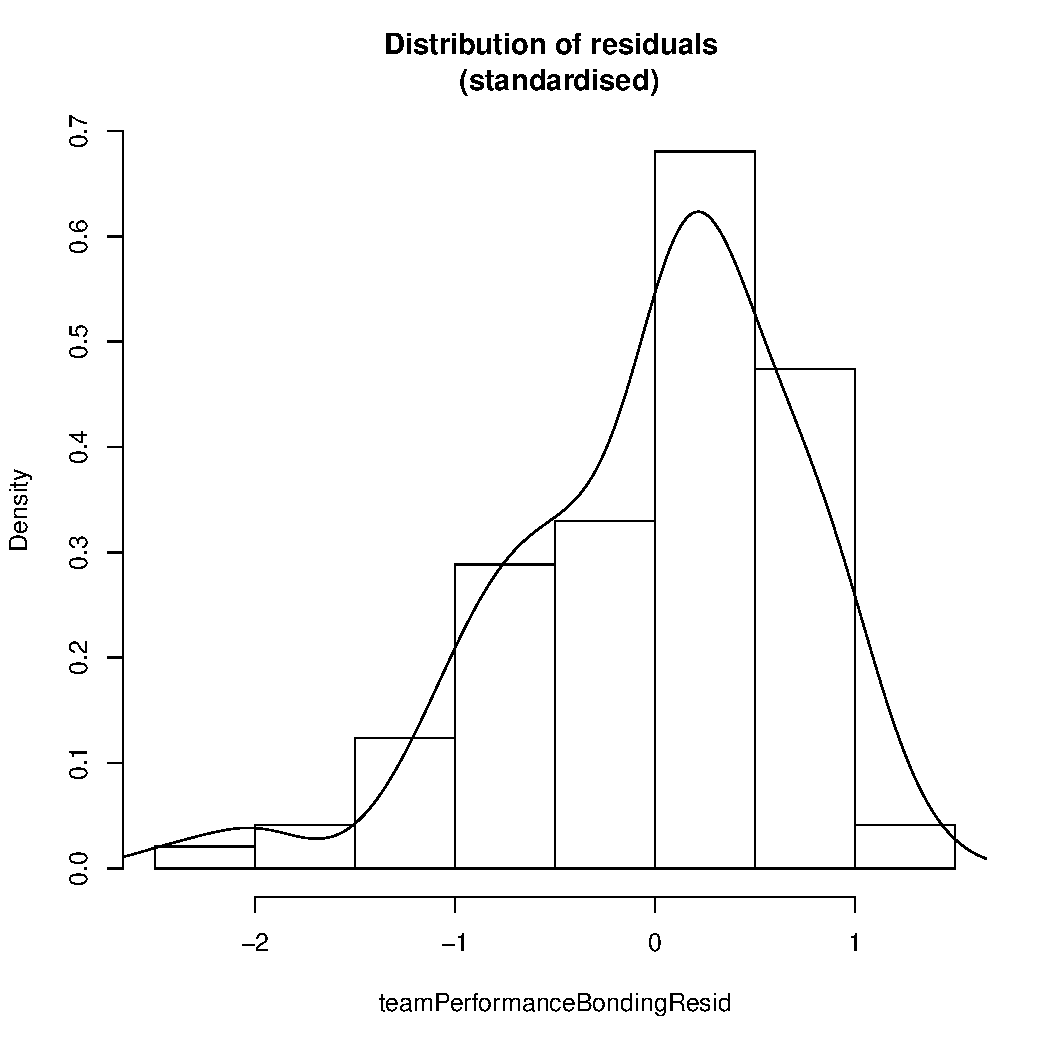
\includegraphics[scale =.4]{images/MLM3aHist.pdf}
  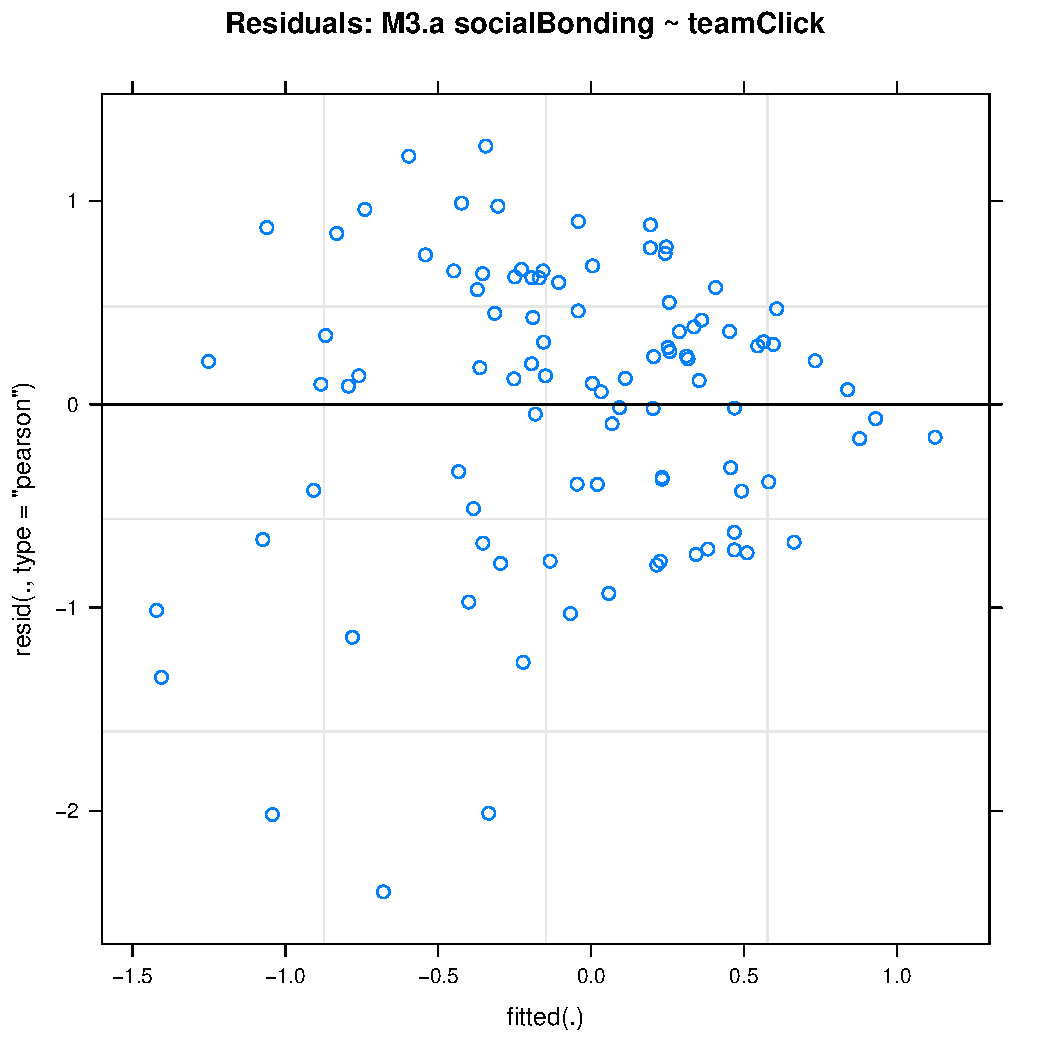
\includegraphics[scale =.4]{images/MLM3aScatter.pdf}
  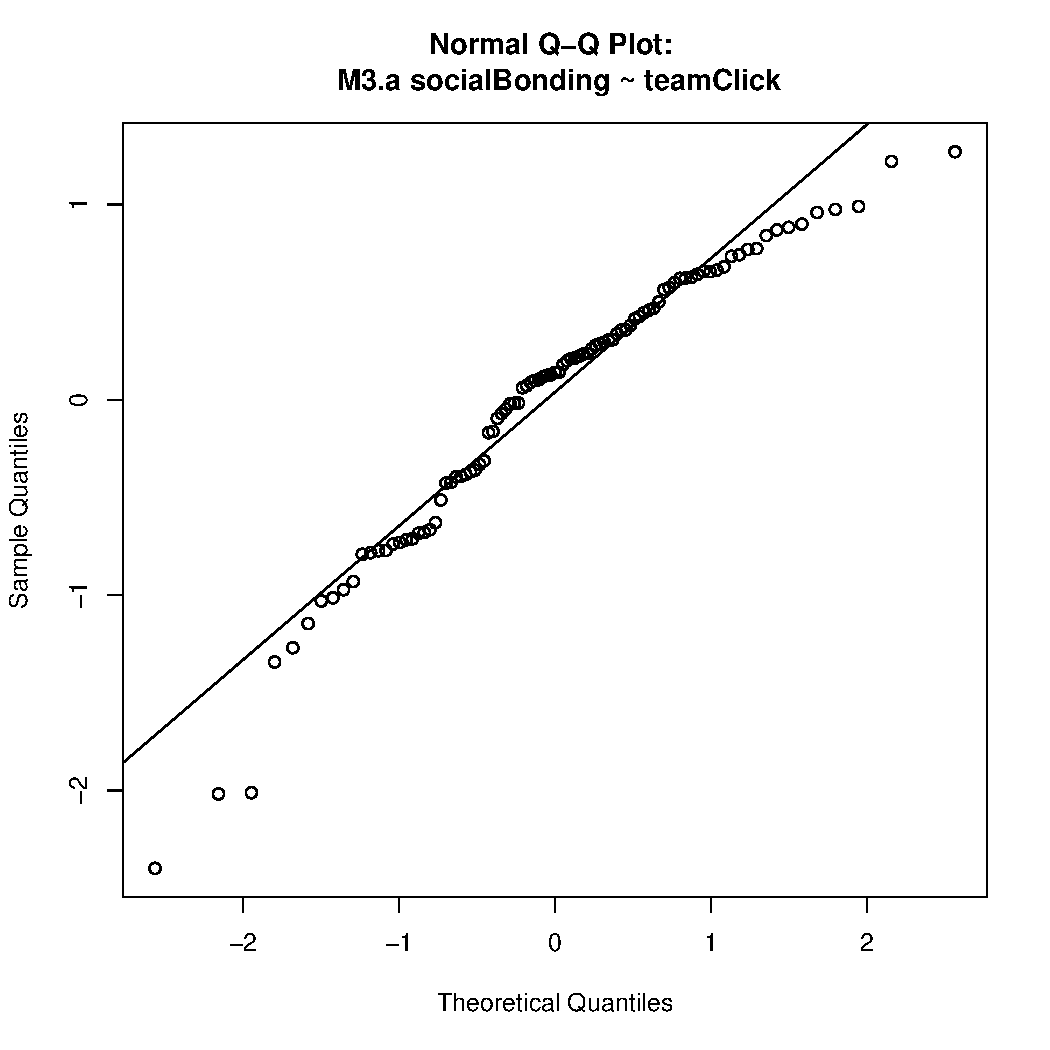
\includegraphics[scale =.4]{images/MLM3aQQNorm.pdf}
  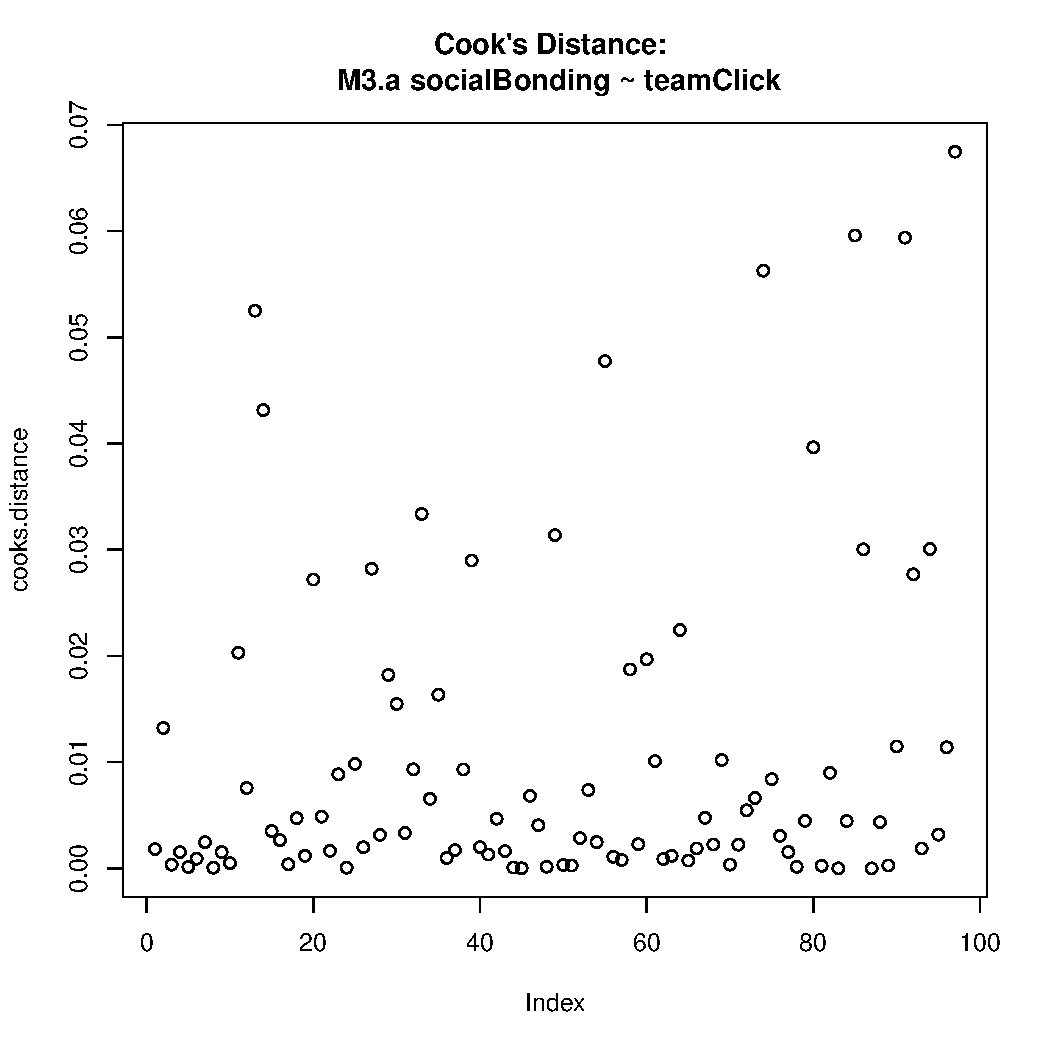
\includegraphics[scale =.4]{images/MLM3aCooksD.pdf}
  \caption{Model Assumptions: M3a Joint Action Success predicts Social Bonding}
  \label{fig:MLM3aAssumptions}
\end{figure}

\begin{figure}[htbp]
  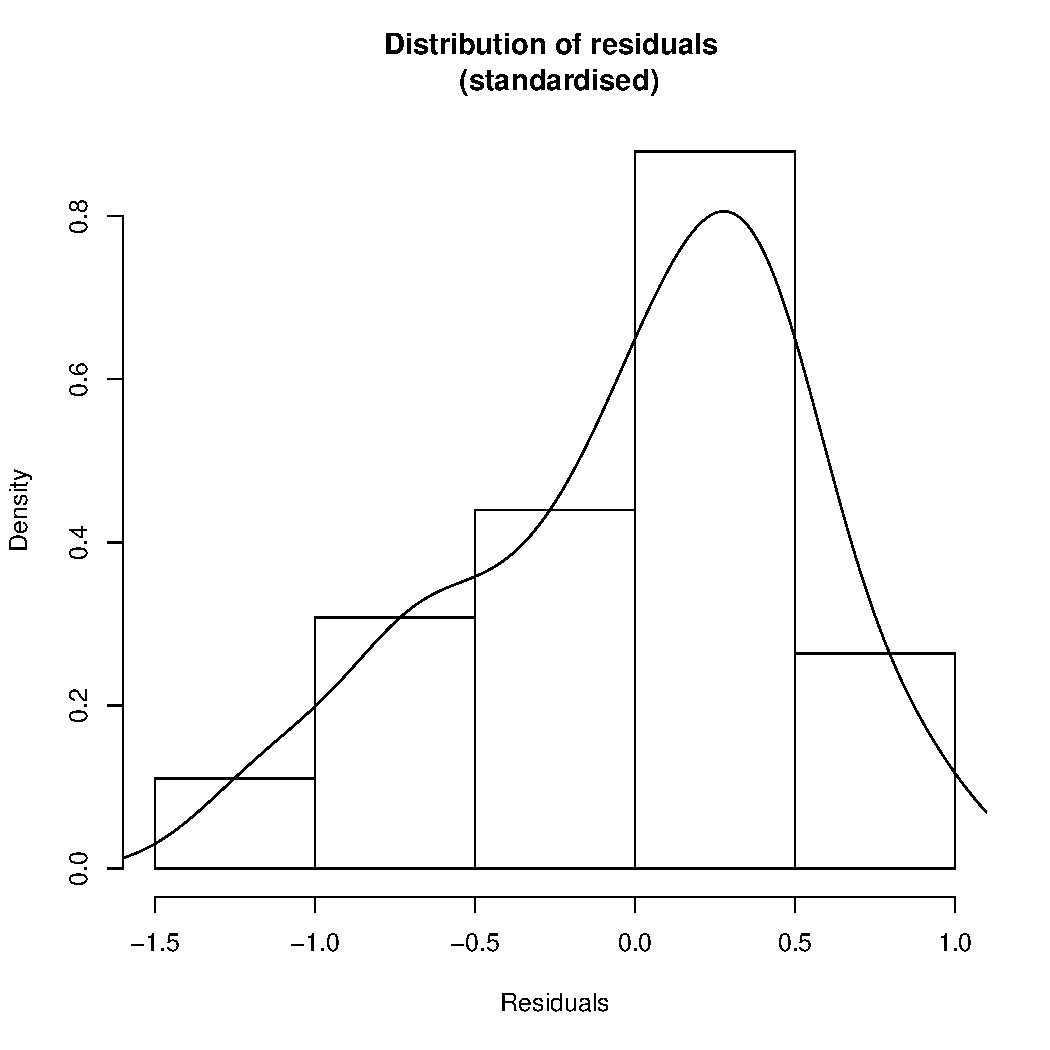
\includegraphics[scale =.4]{images/MLM3aOutHist.pdf}
  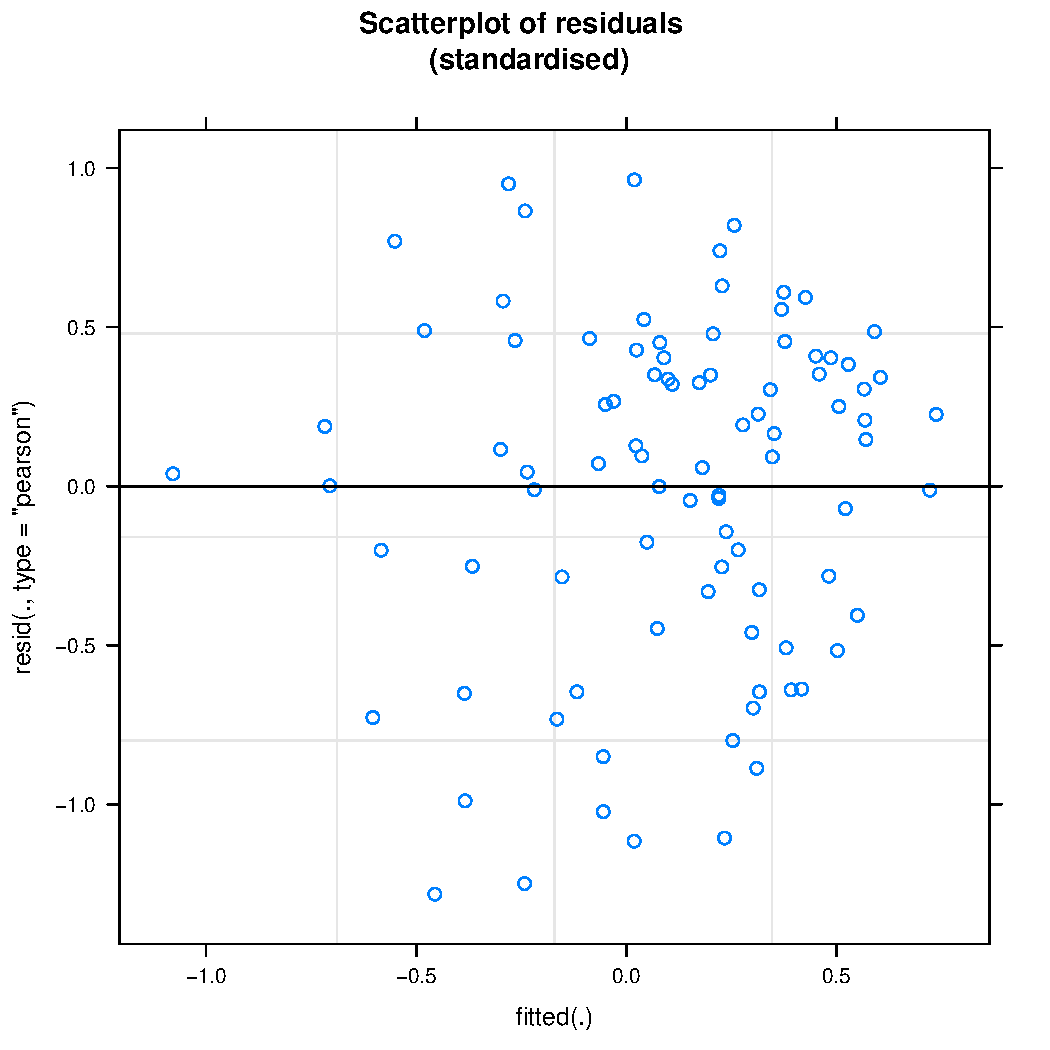
\includegraphics[scale =.4]{images/MLM3aOutScatter.pdf}
  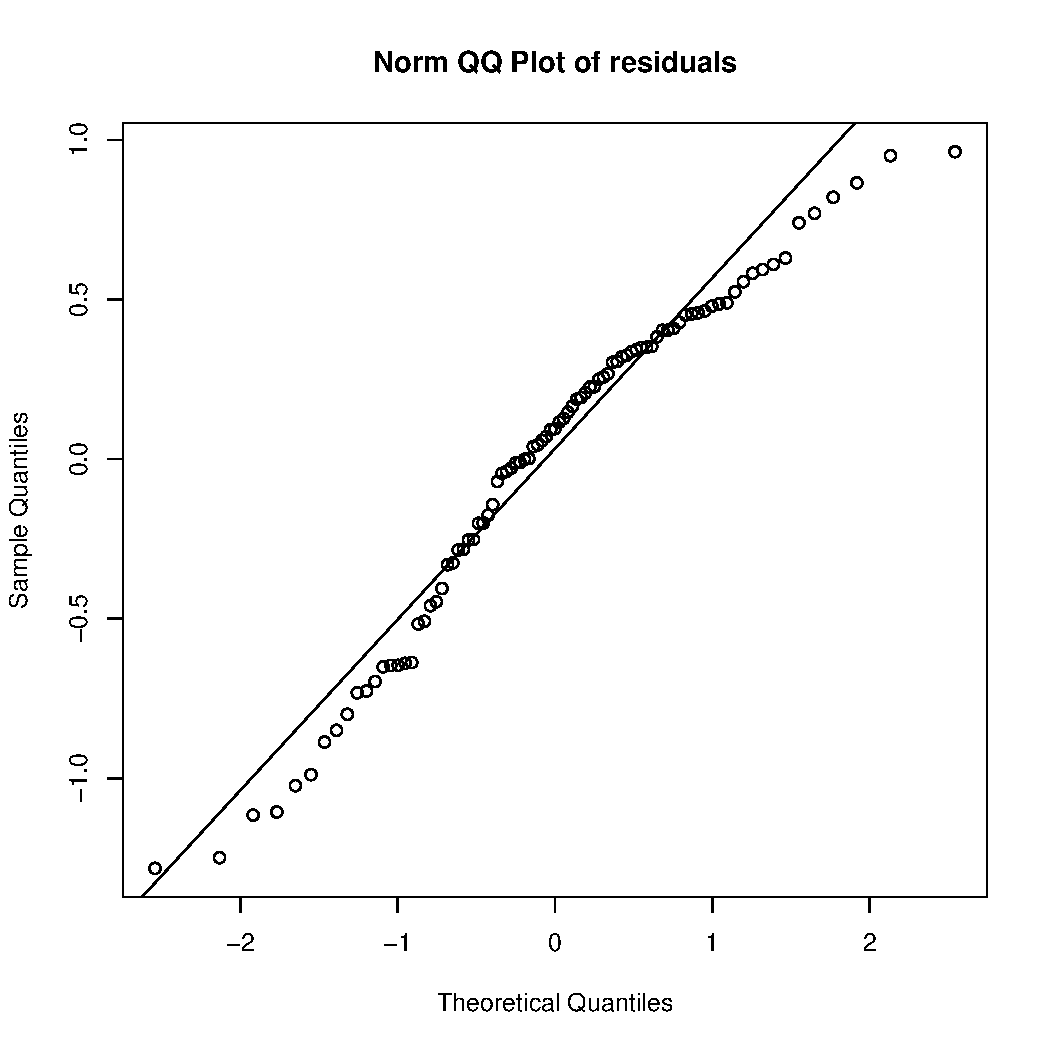
\includegraphics[scale =.4]{images/MLM3aOutQQNorm.pdf}
  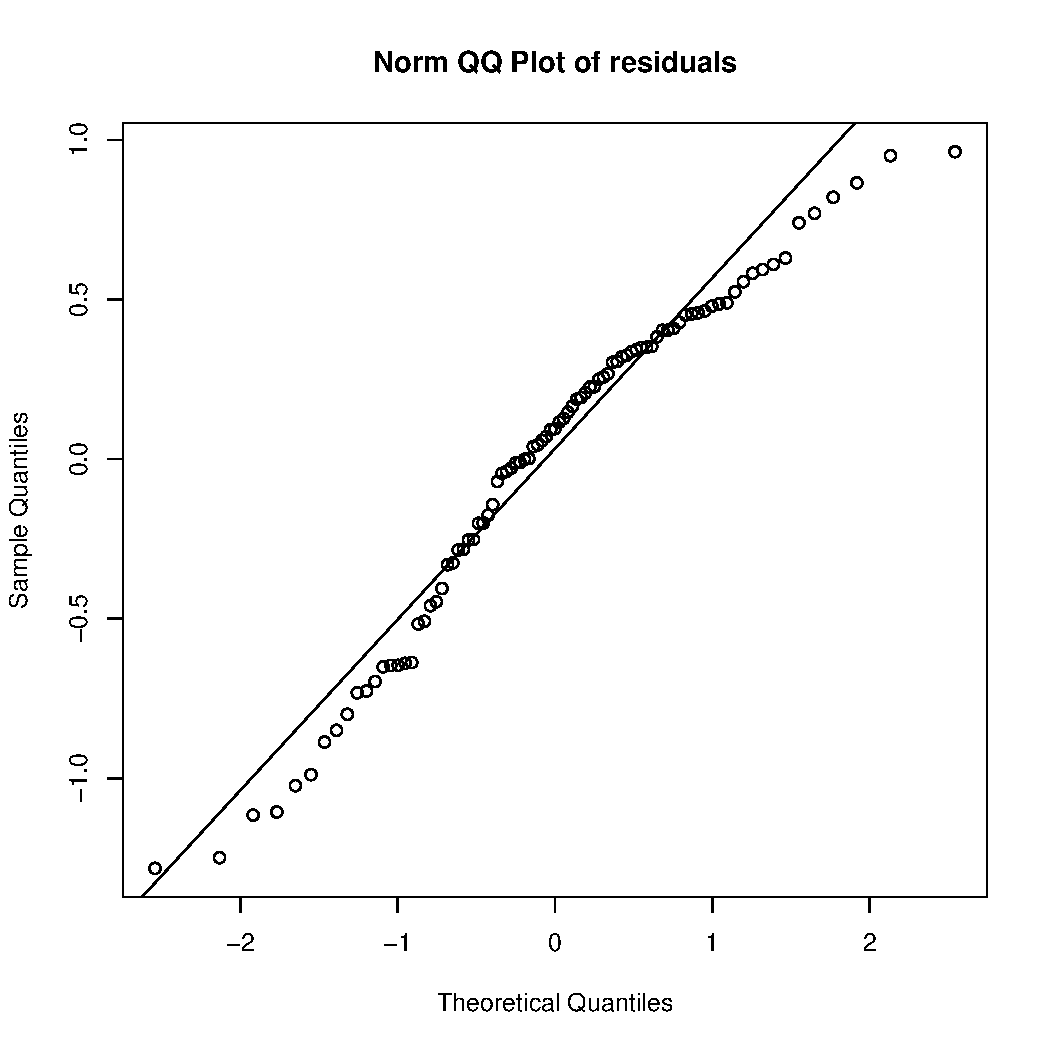
\includegraphics[scale =.4]{images/MLM3aOutCooksD.pdf}
  \caption{Model Assumptions: M3a Joint Action Success predicts Social Bonding (outliers removed)}
  \label{fig:MLM3aOutAssumptions}
\end{figure}

\begin{figure}[htbp]
  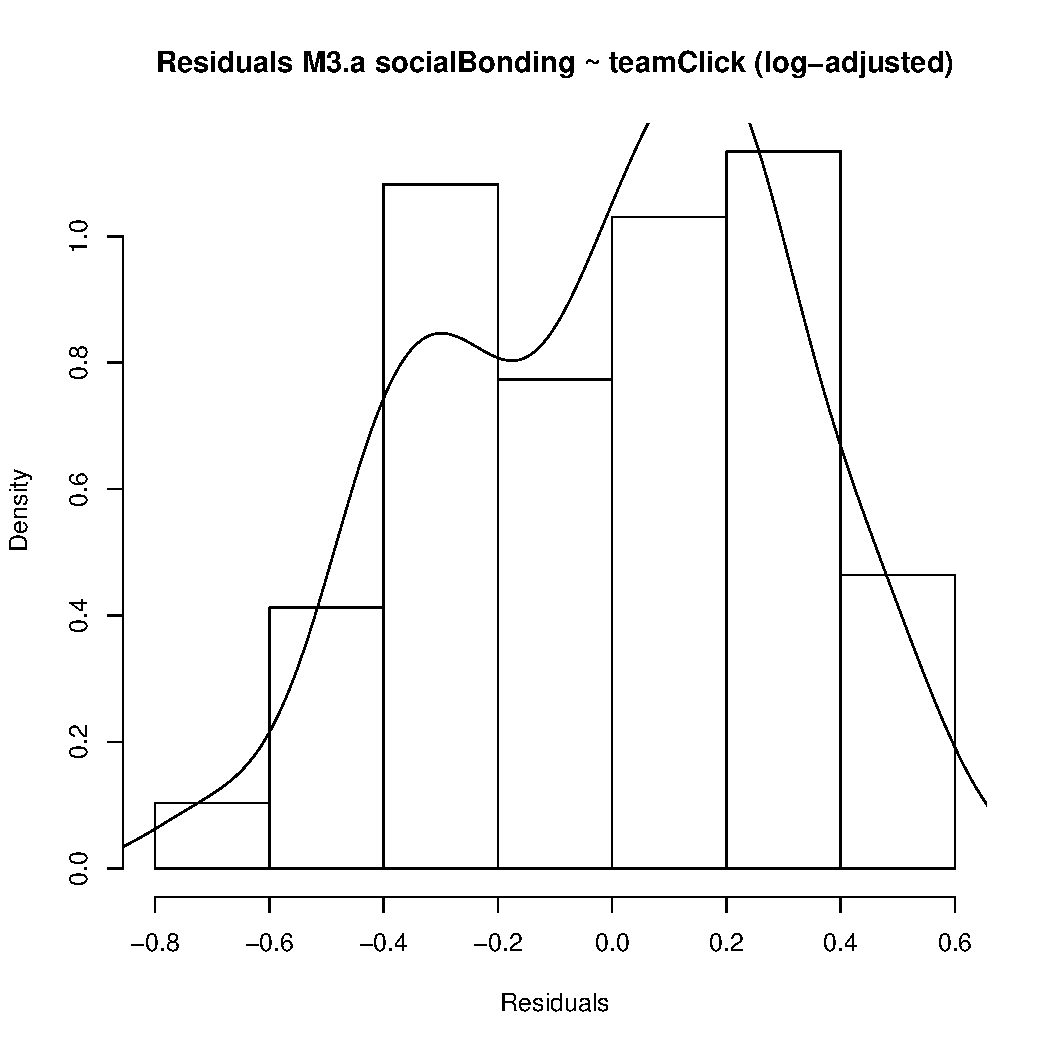
\includegraphics[scale =.4]{images/MLM3aLogHist.pdf}
  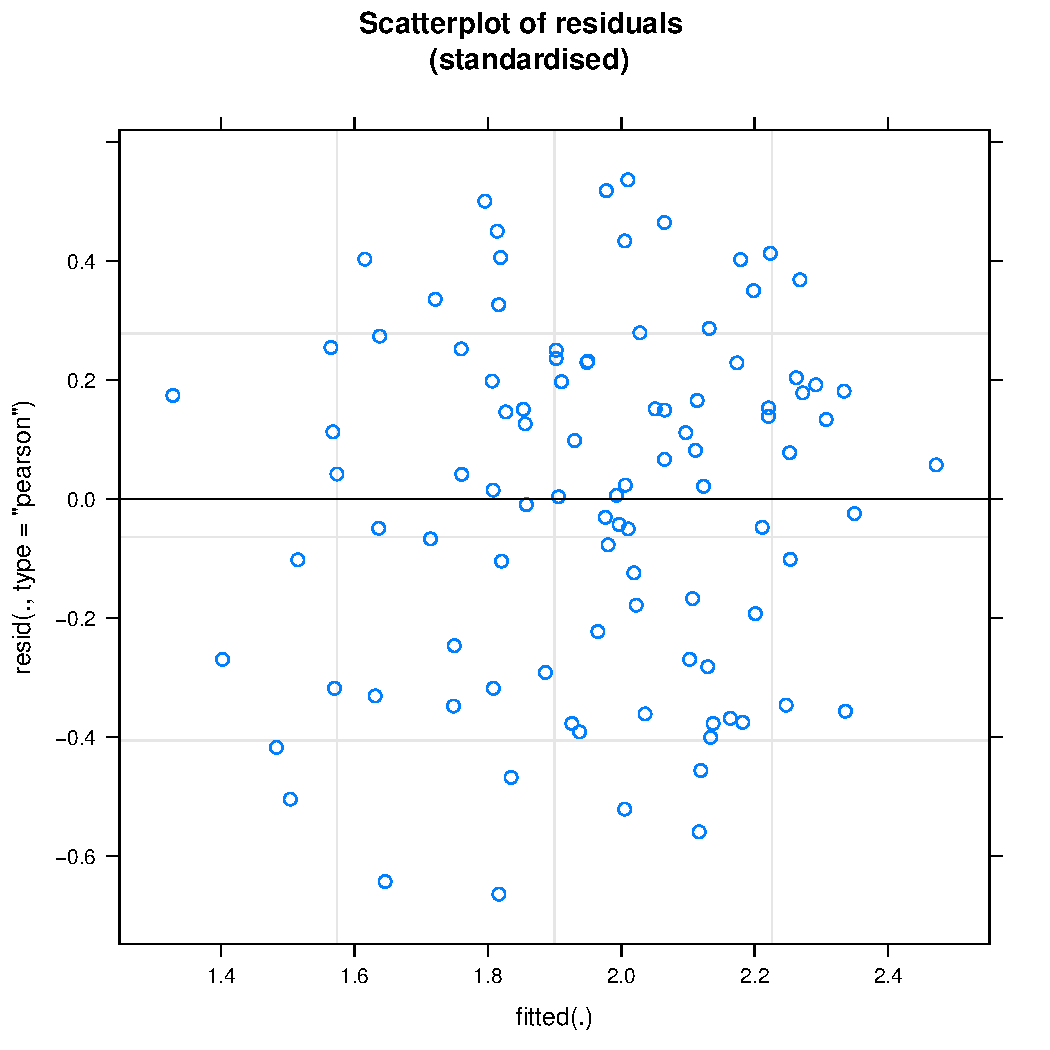
\includegraphics[scale =.4]{images/MLM3aLogScatter.pdf}
  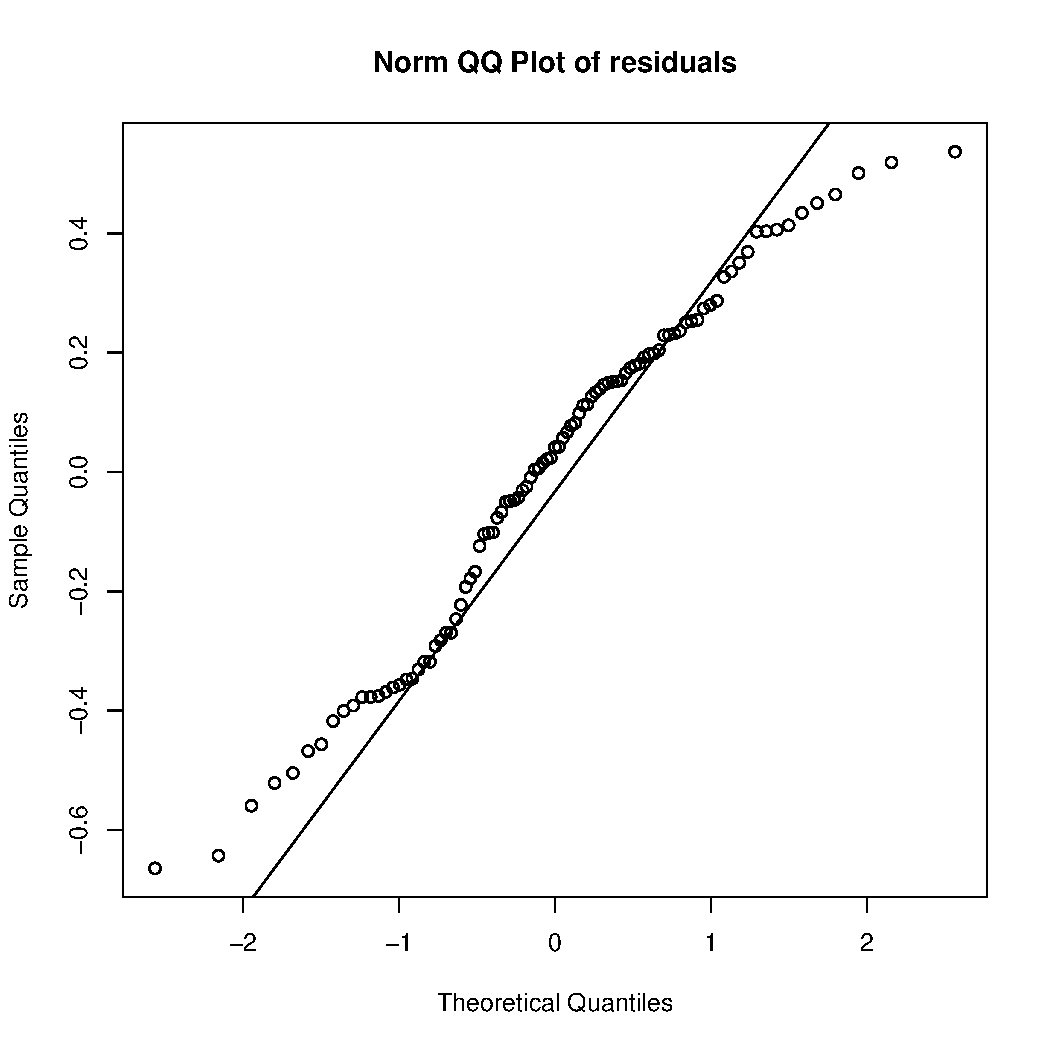
\includegraphics[scale =.4]{images/MLM3aLogQQNorm.pdf}
  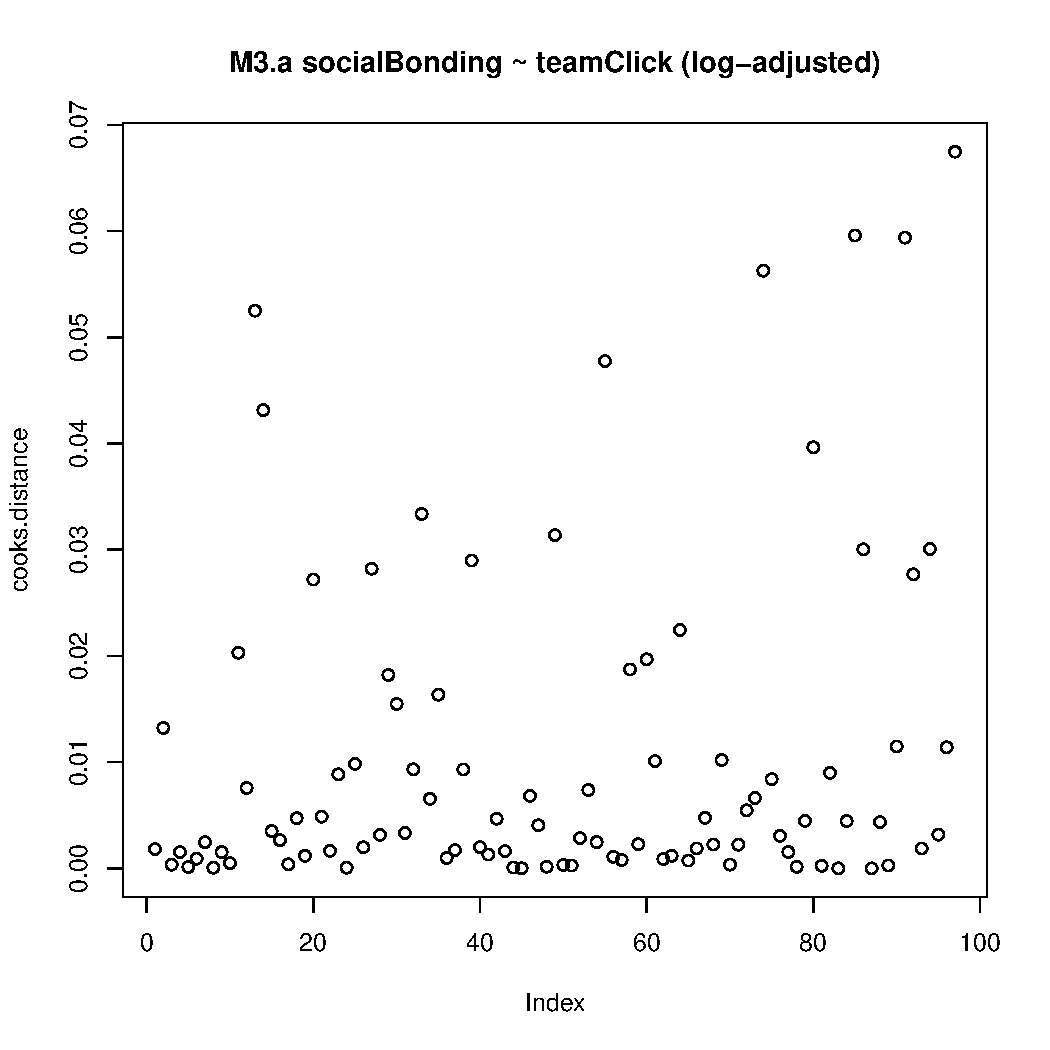
\includegraphics[scale =.4]{images/MLM3aLogCooksD.pdf}
  \caption{Model Assumptions: M3a Joint Action Success predicts Social Bonding (log-transformed)}
  \label{fig:MLM3aLogAssumptions}
\end{figure}








\begin{figure}[htbp]
  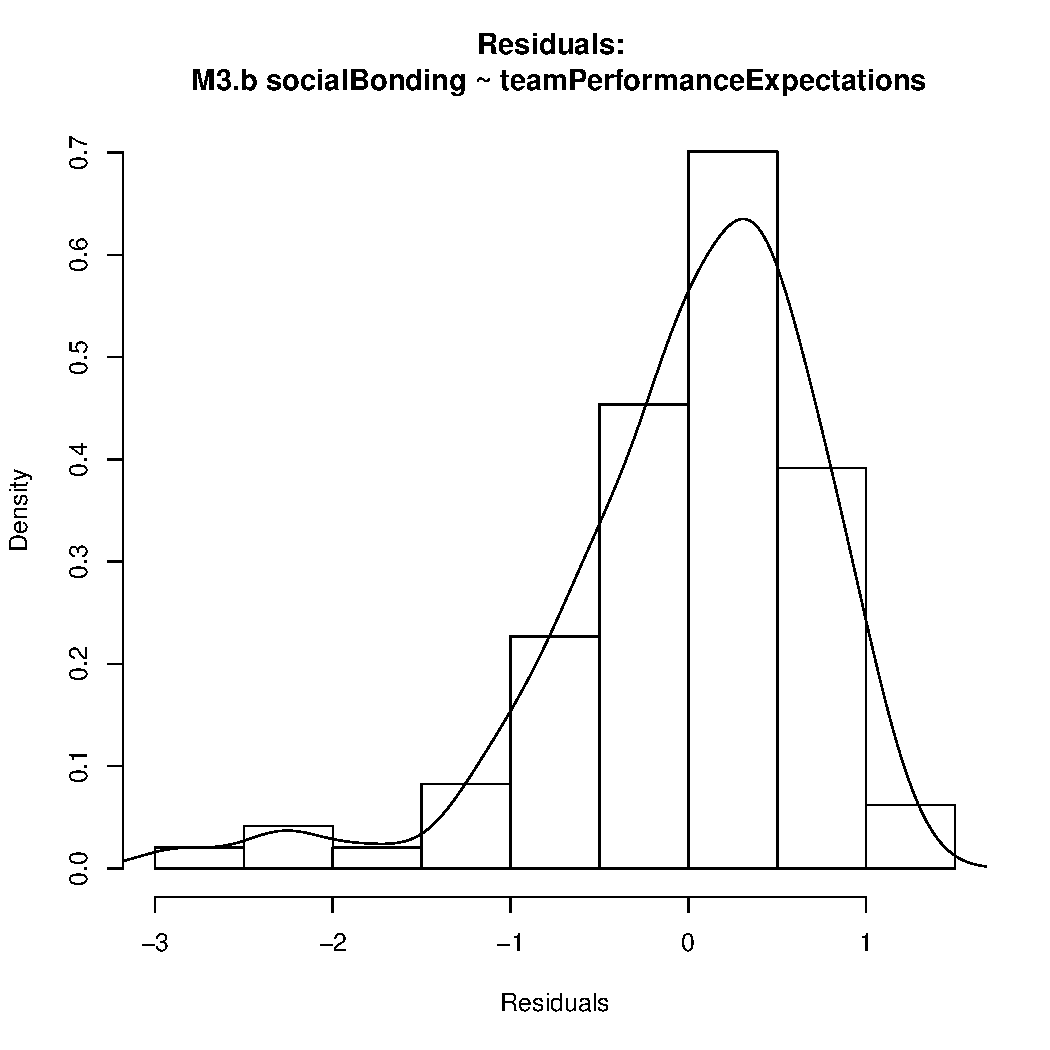
\includegraphics[scale =.4]{images/MLM3bHist.pdf}
  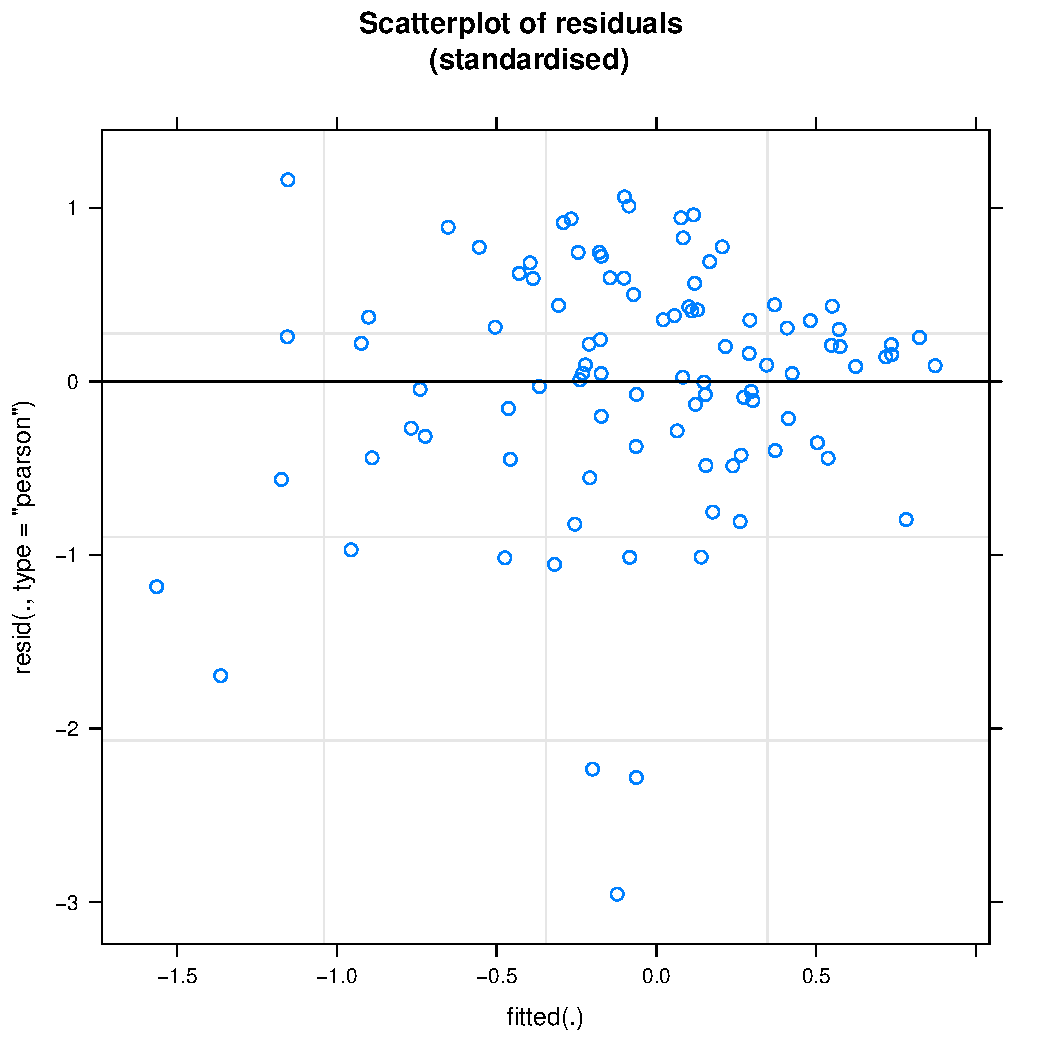
\includegraphics[scale =.4]{images/MLM3bScatter.pdf}
  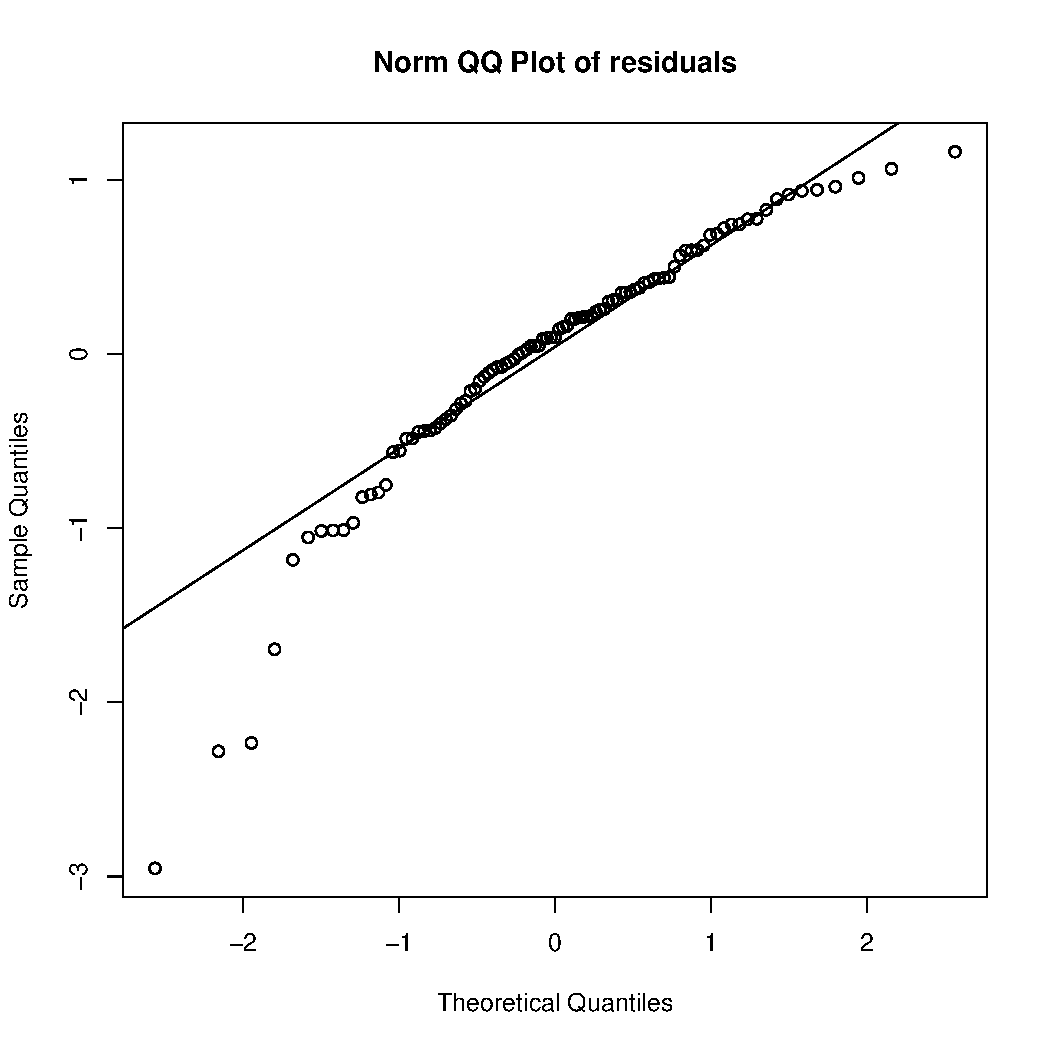
\includegraphics[scale =.4]{images/MLM3bQQNorm.pdf}
  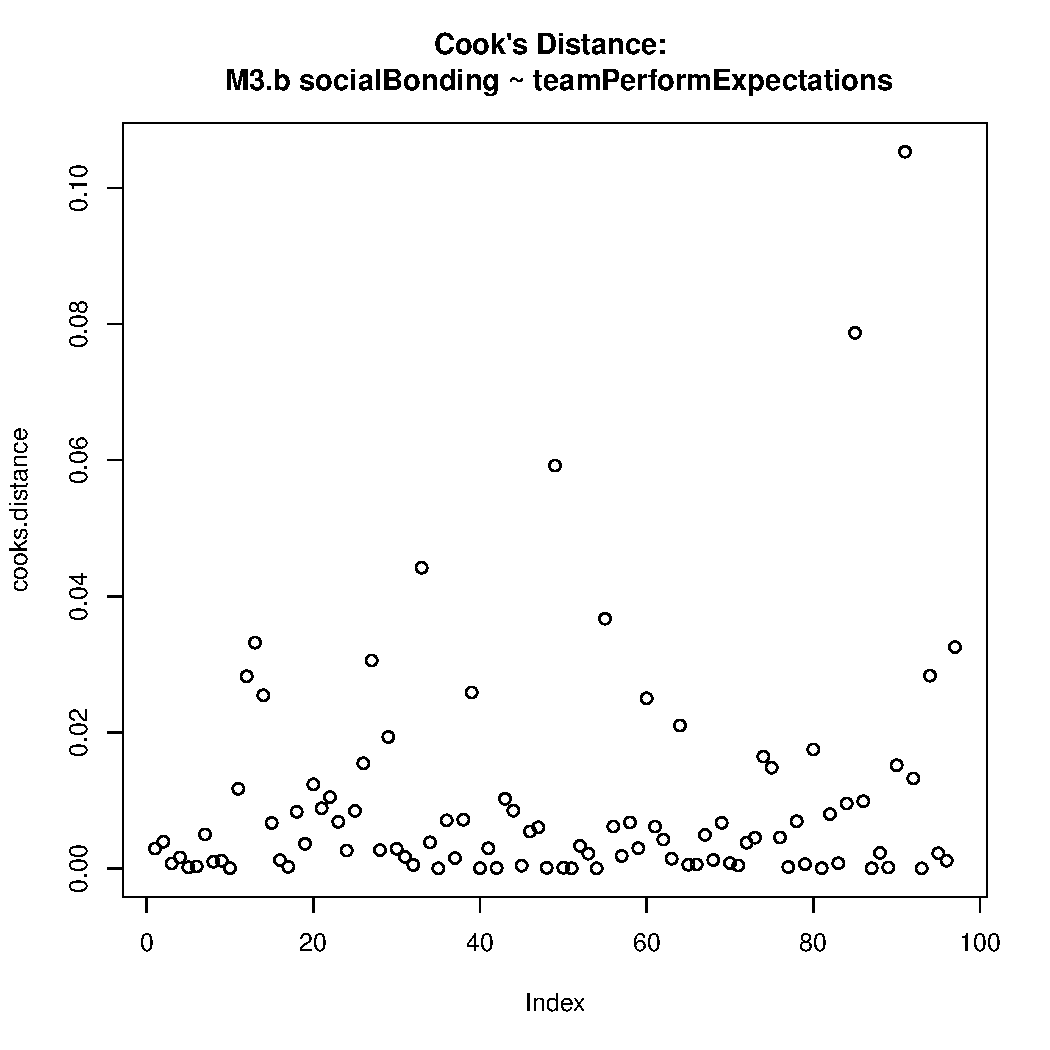
\includegraphics[scale =.4]{images/MLM3bCooksD.pdf}
  \caption{Model Assumptions: M3a Joint Action Success predicts Social Bonding (log-transformed)}
  \label{fig:MLM3bAssumptions}
\end{figure}

\begin{figure}[htbp]
  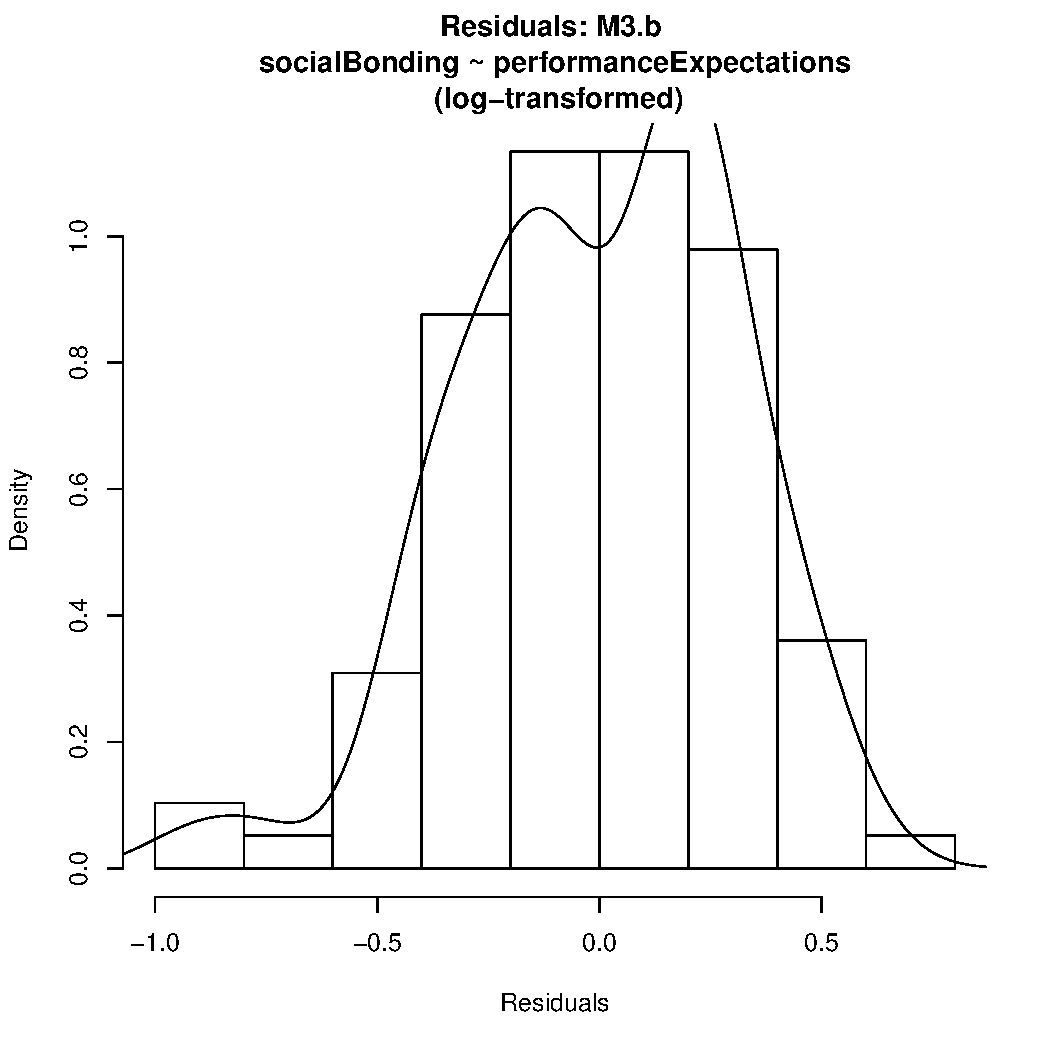
\includegraphics[scale =.4]{images/MLM3bLogHist.pdf}
  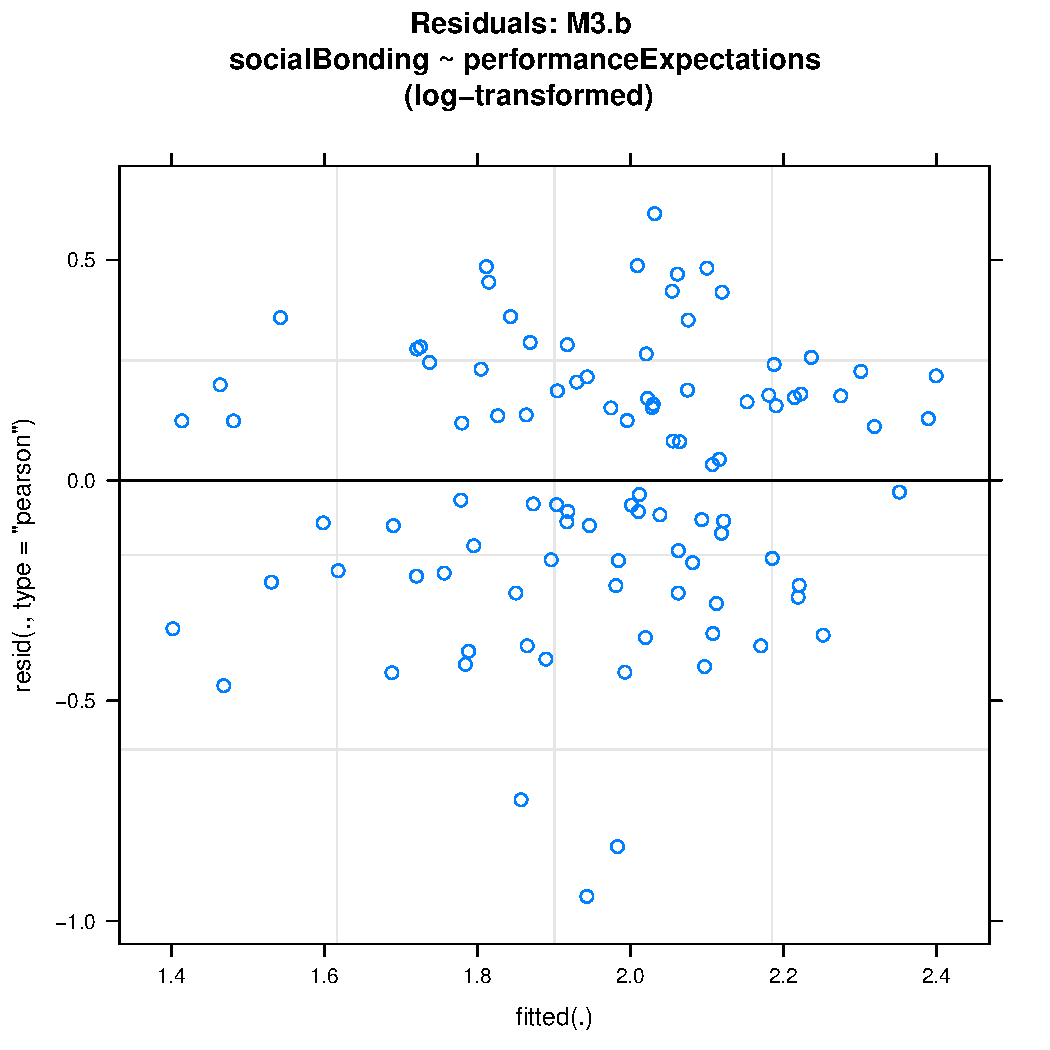
\includegraphics[scale =.4]{images/MLM3bLogScatter.pdf}
  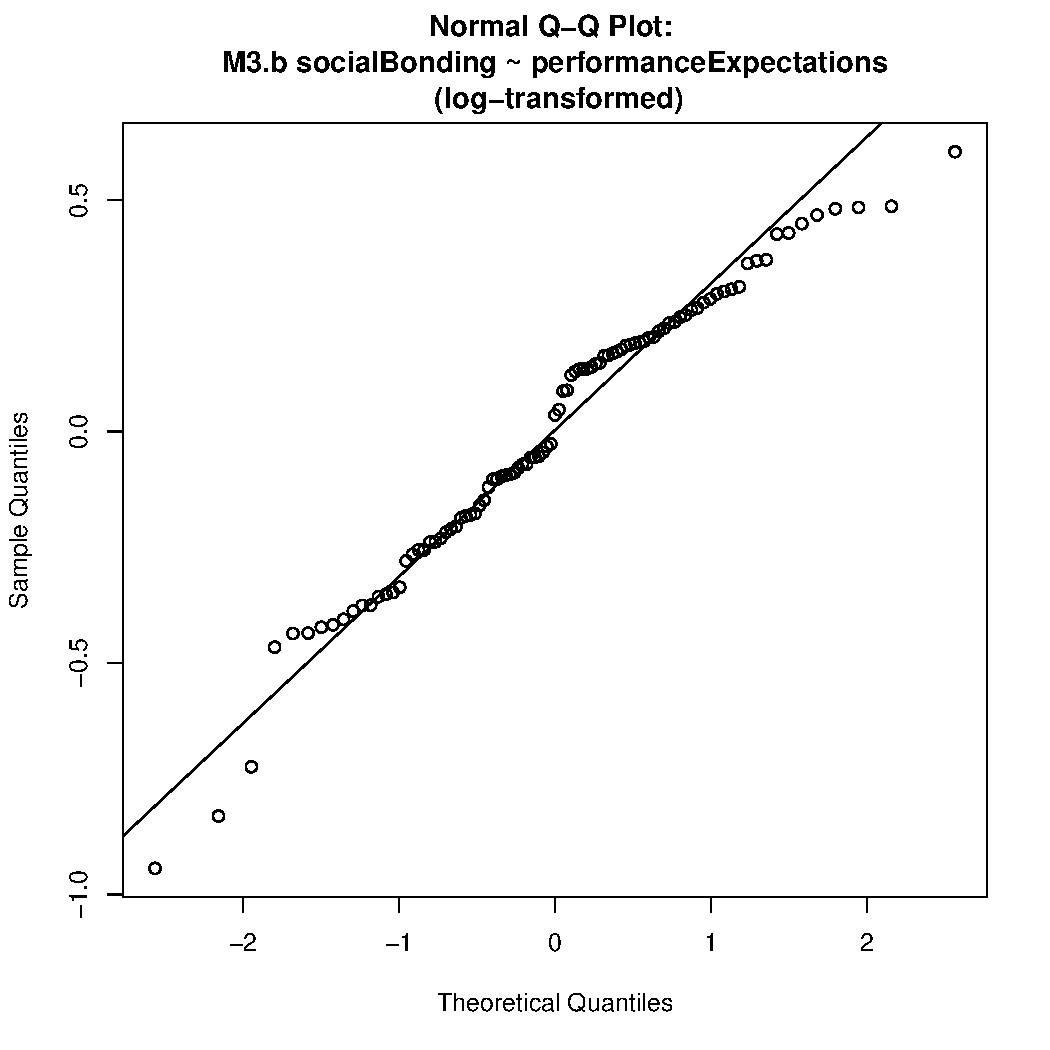
\includegraphics[scale =.4]{images/MLM3bLogQQNorm.pdf}
  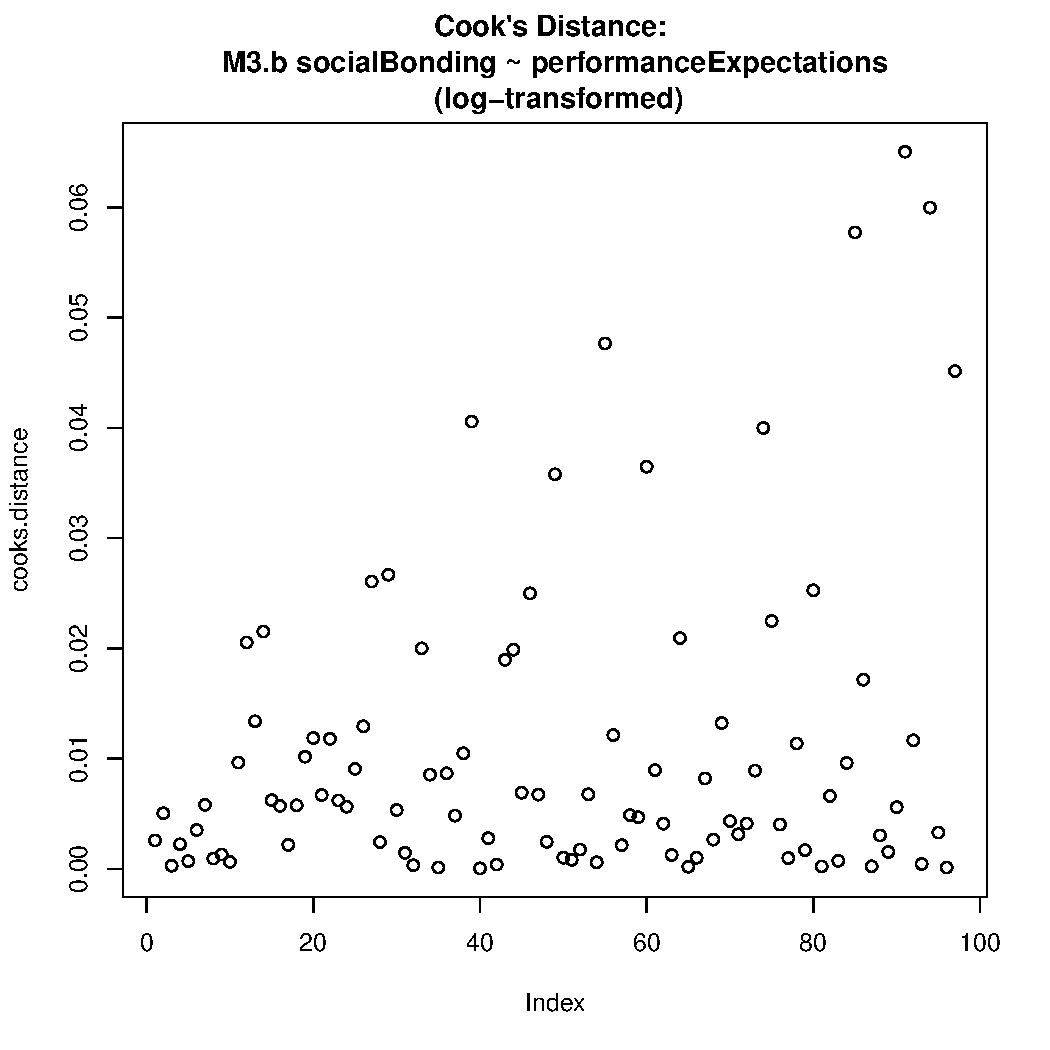
\includegraphics[scale =.4]{images/MLM3bLogCooksD.pdf}
  \caption{Model Assumptions: M3a Joint Action Success predicts Social Bonding (log-transformed)}
  \label{fig:MLM3bLogAssumptions}
\end{figure}






\begin{figure}[htbp]
  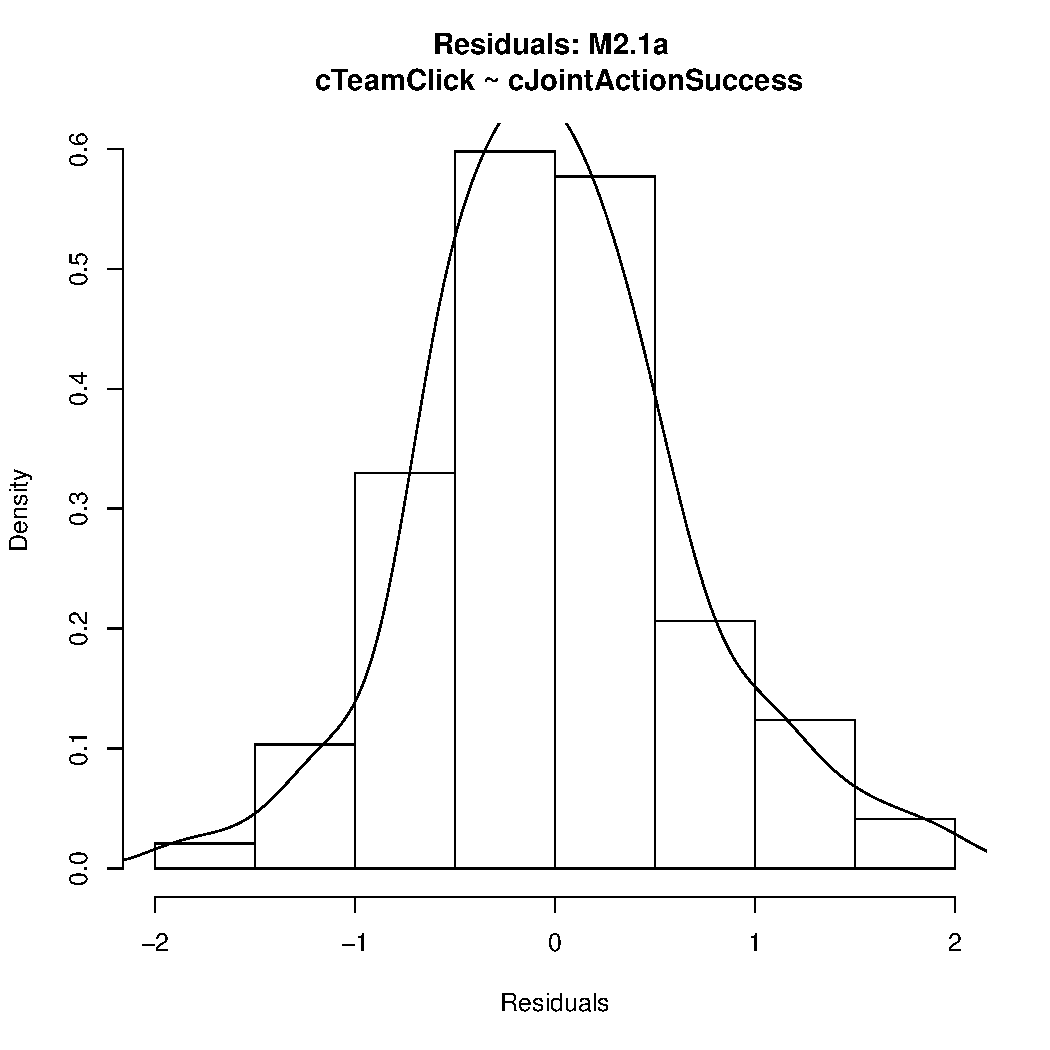
\includegraphics[scale =.4]{images/MLM21aHist.pdf}
  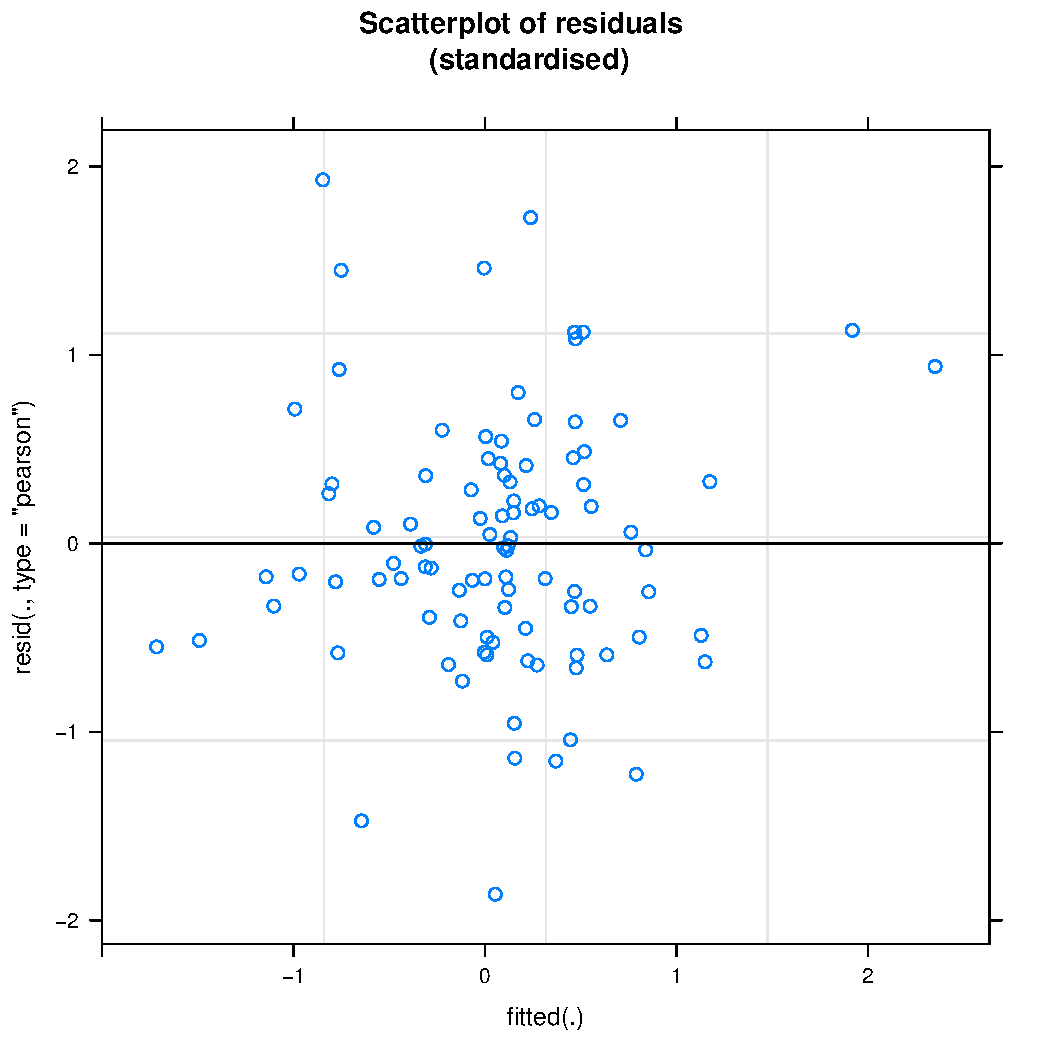
\includegraphics[scale =.4]{images/MLM21aScatter.pdf}
  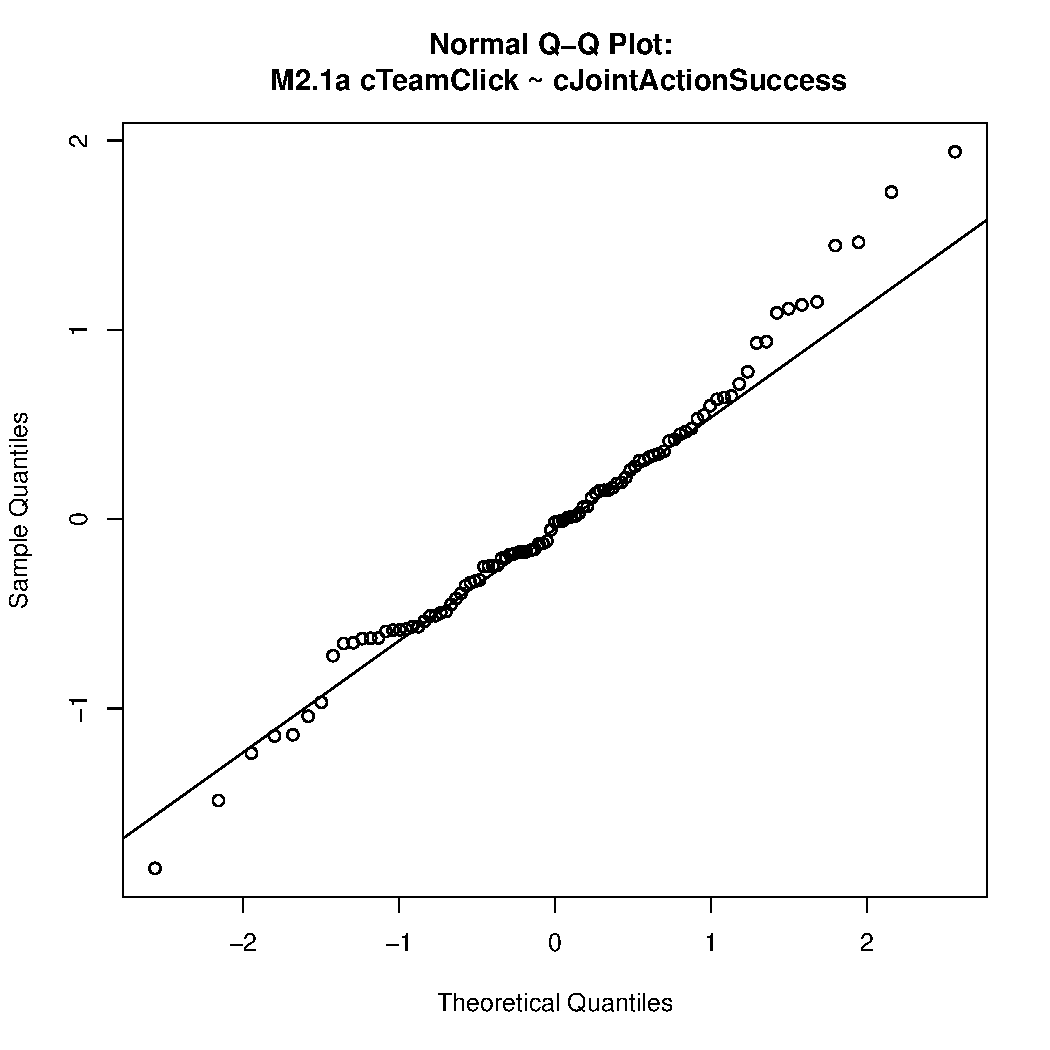
\includegraphics[scale =.4]{images/MLM21aQQNorm.pdf}
  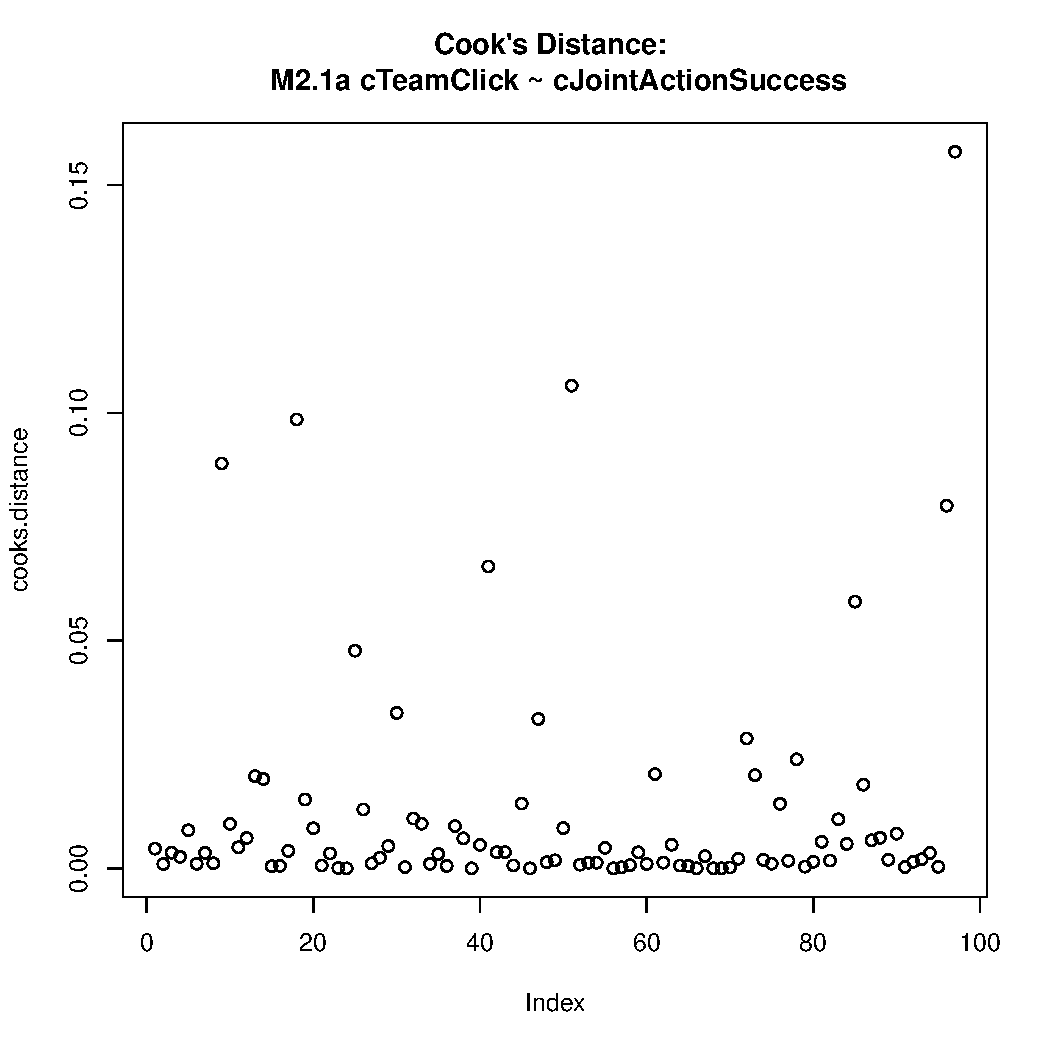
\includegraphics[scale =.4]{images/MLM21aCooksD.pdf}
  \caption{Model Assumptions: M2.1a Change in Joint Action Success predicts change in Team Click}
  \label{fig:MLM21aAssumptions}
\end{figure}





\begin{figure}[htbp]
  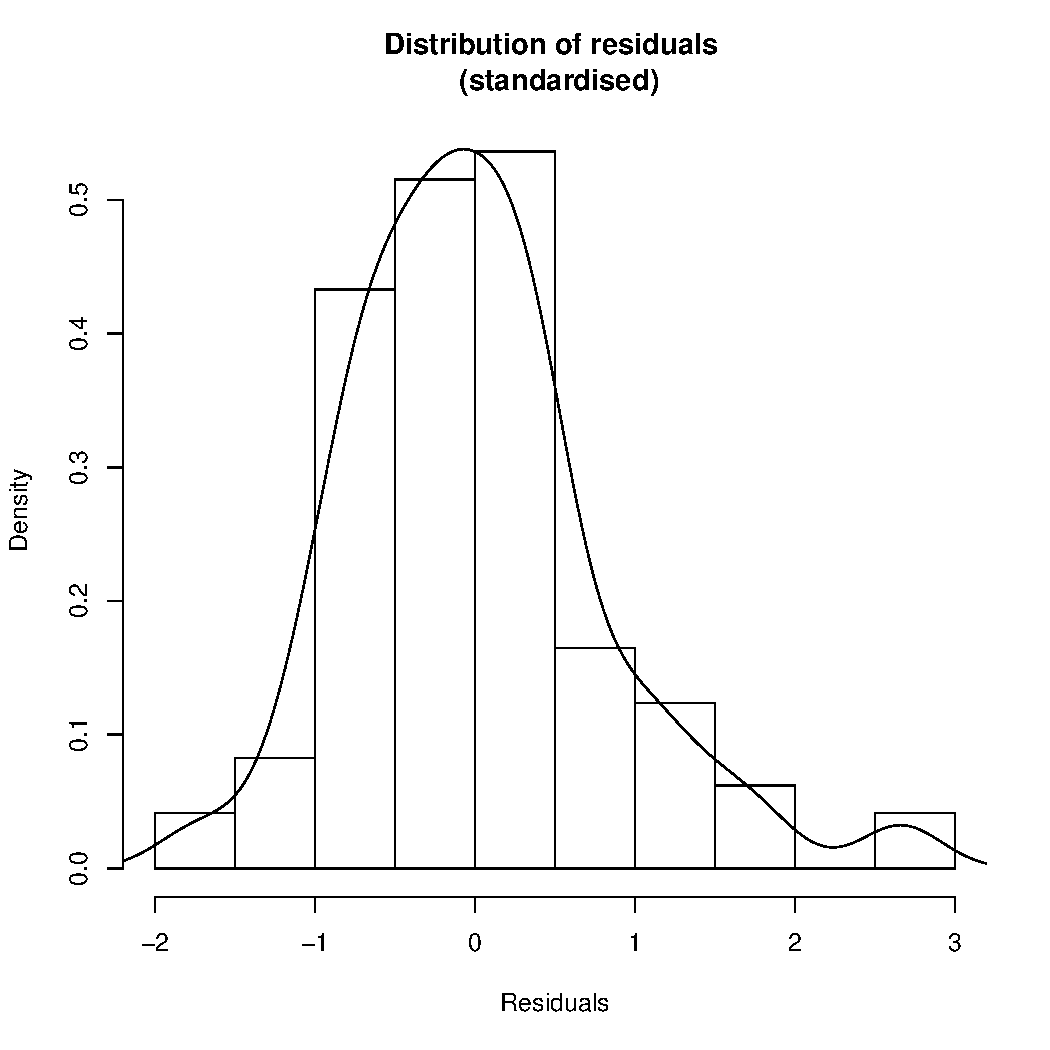
\includegraphics[scale =.4]{images/MLM21bHist.pdf}
  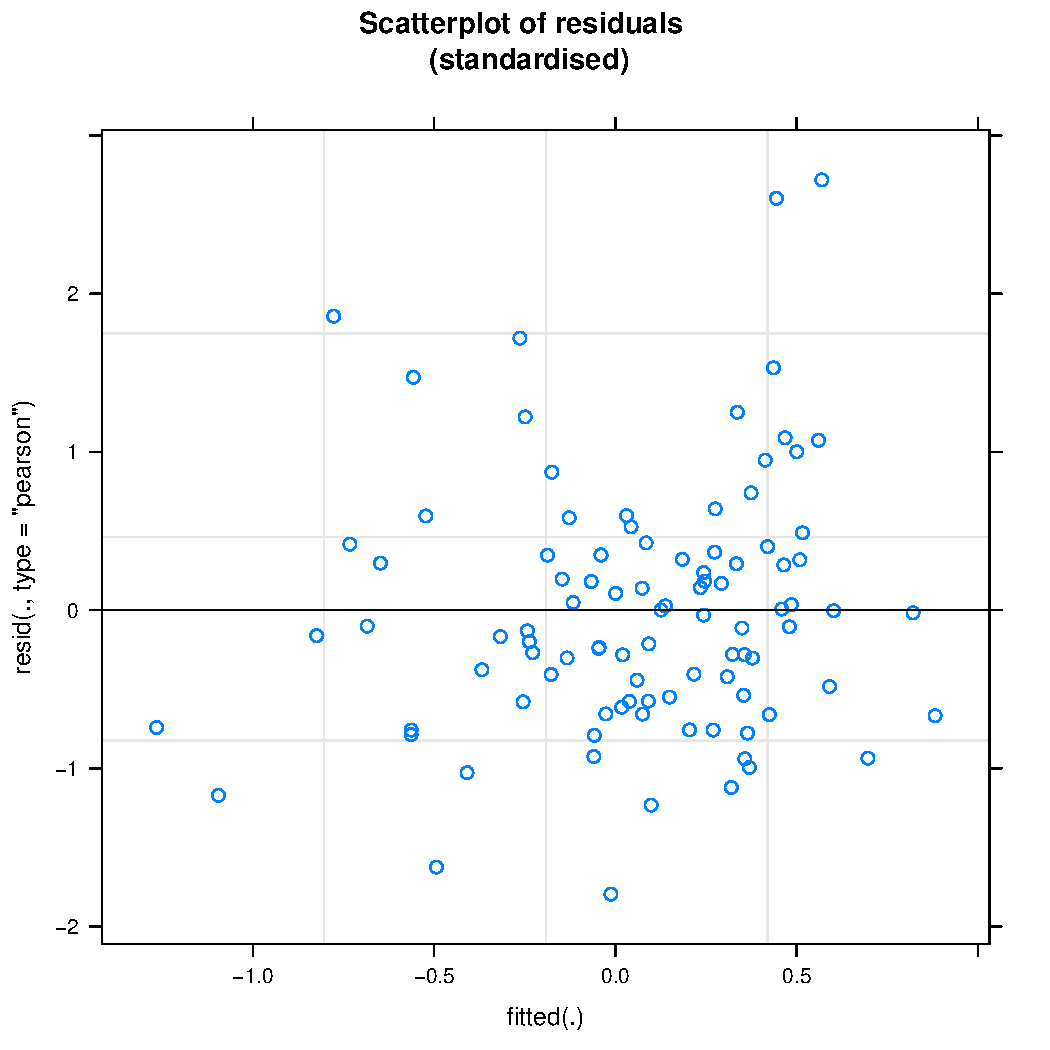
\includegraphics[scale =.4]{images/MLM21bScatter.pdf}
  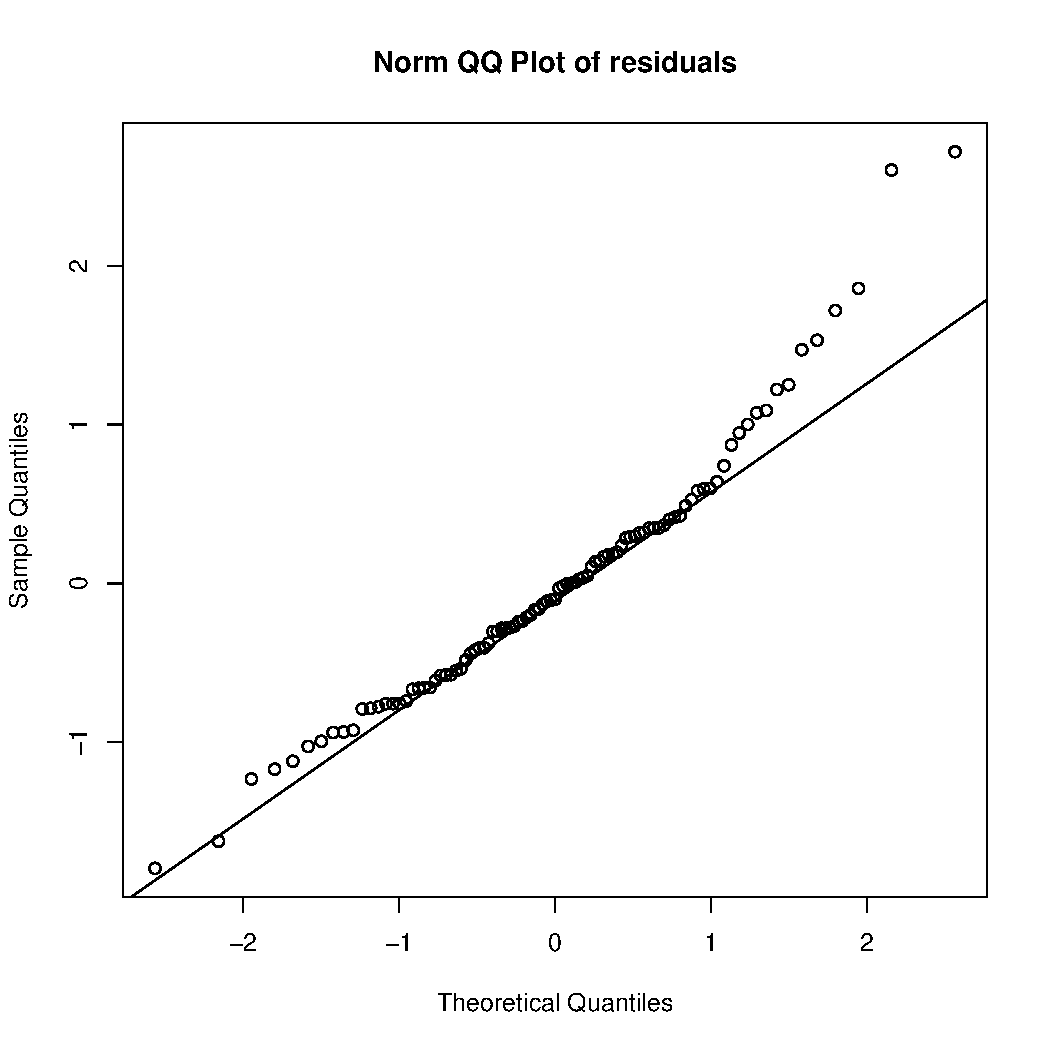
\includegraphics[scale =.4]{images/MLM21bQQNorm.pdf}
  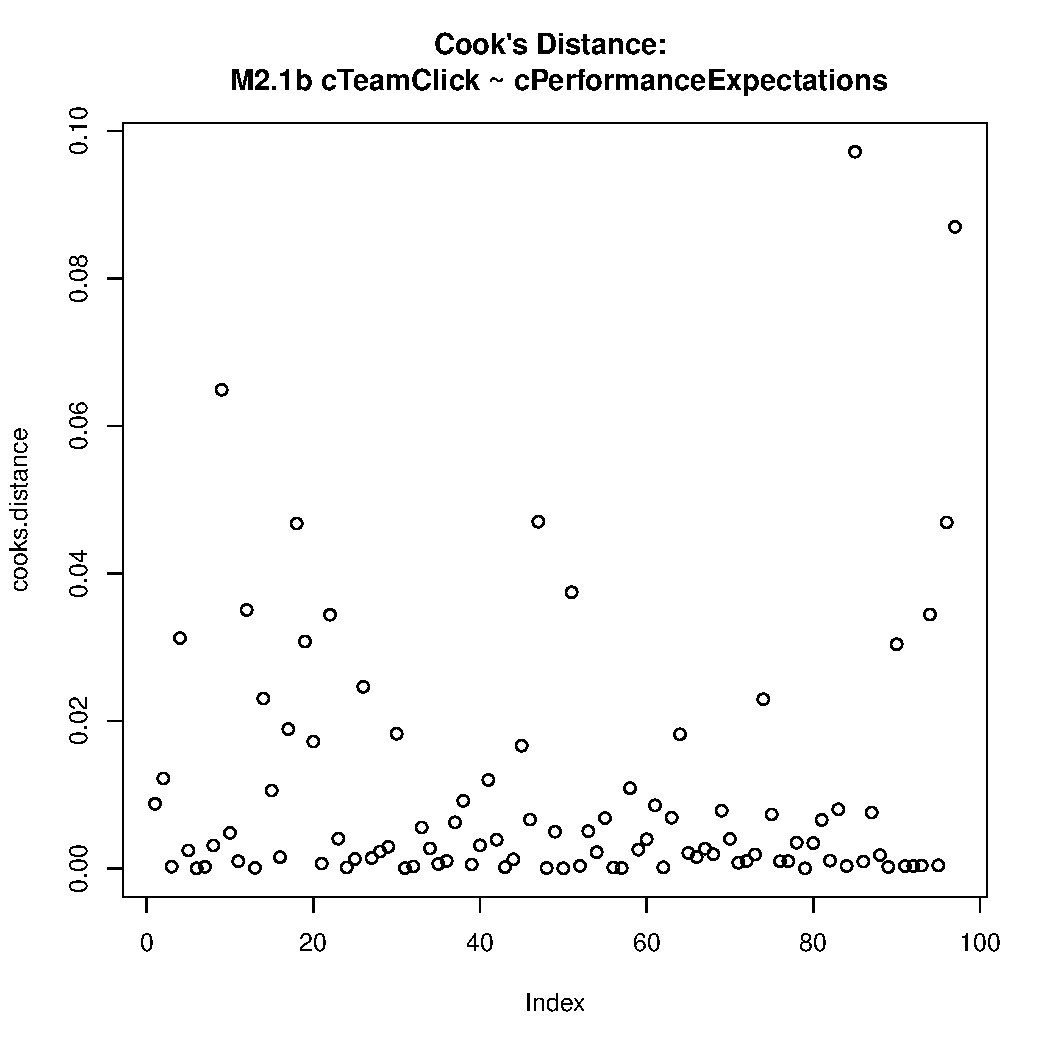
\includegraphics[scale =.4]{images/MLM21bCooksD.pdf}
  \caption{Model Assumptions: M2.1b Team Performance Expectations post-Tournament predicts change in Team Click}
  \label{fig:MLM21bAssumptions}
\end{figure}


\begin{figure}[htbp]
  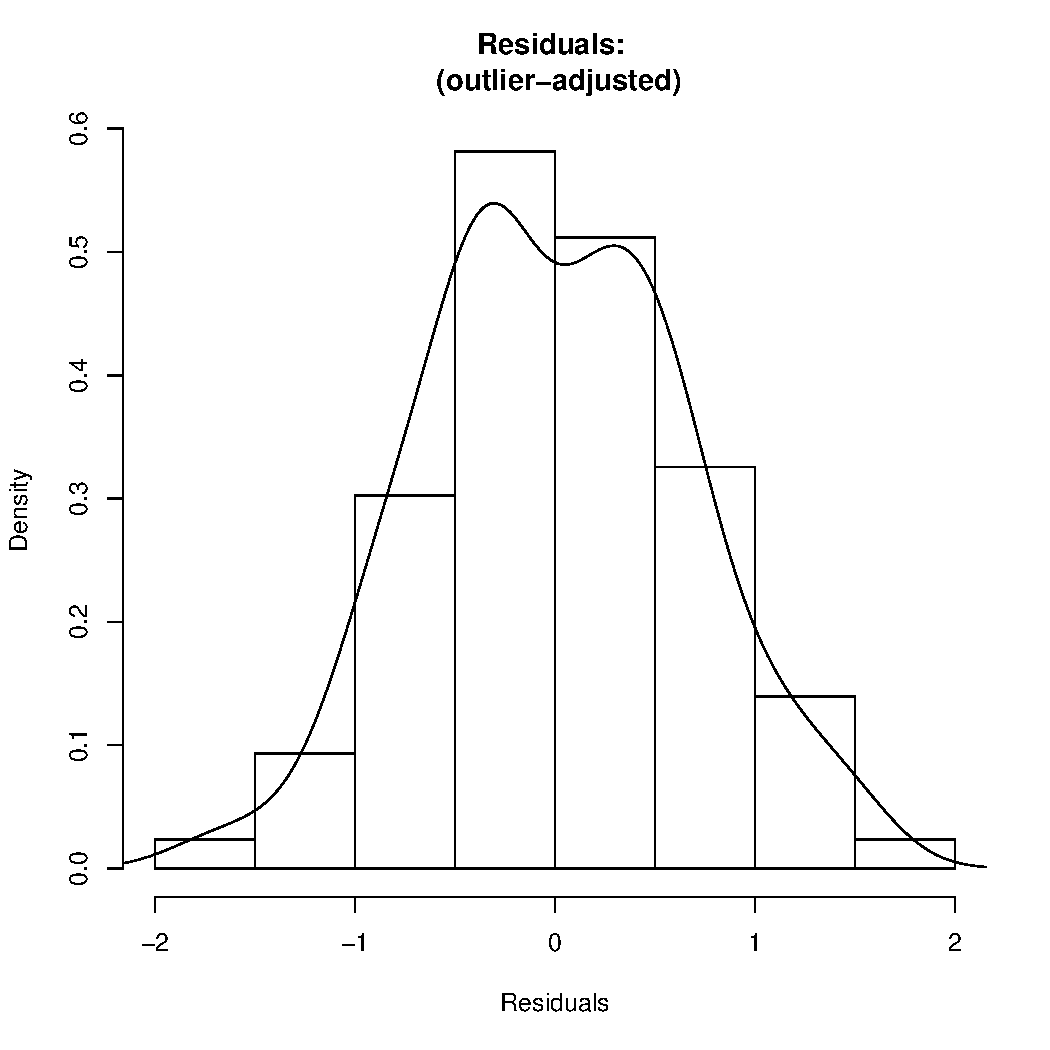
\includegraphics[scale =.4]{images/MLM21bOutHist.pdf}
  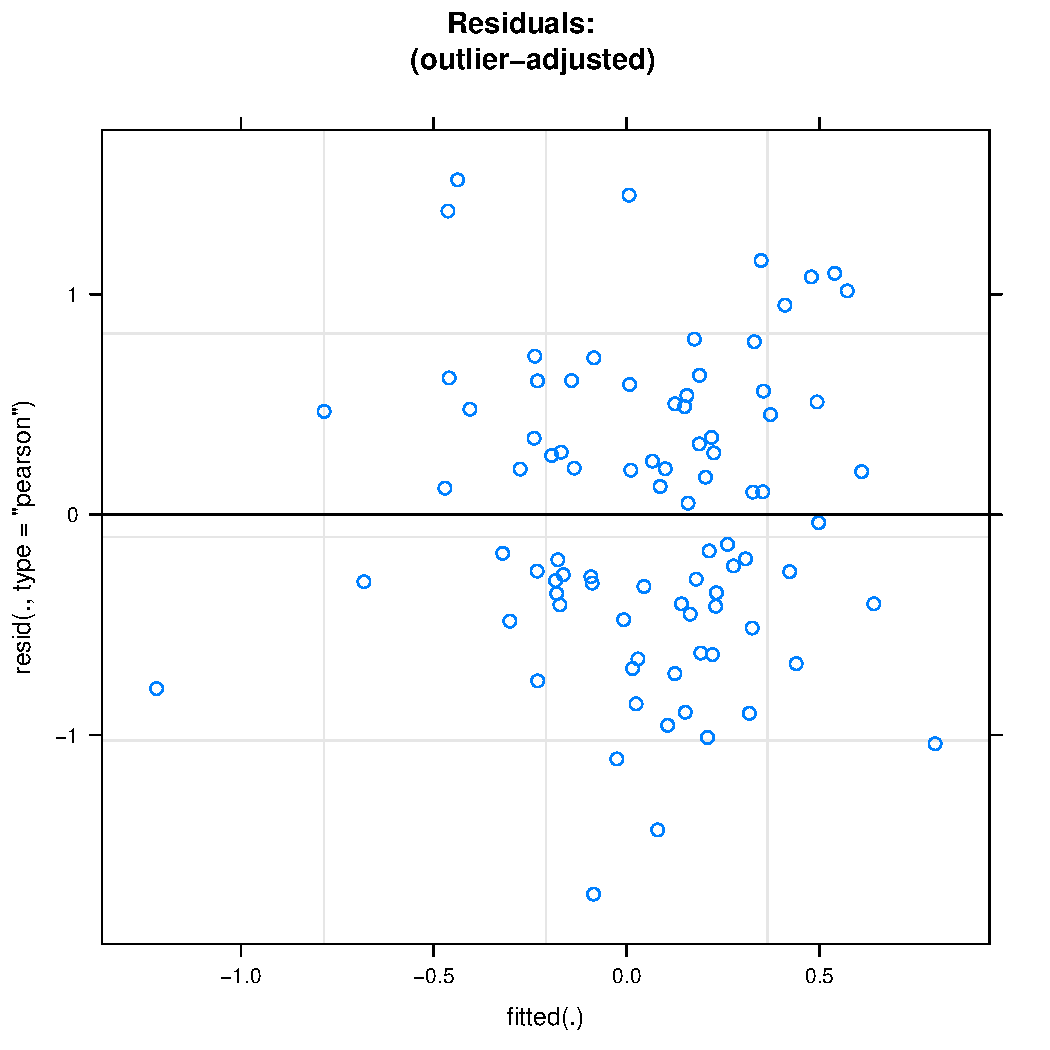
\includegraphics[scale =.4]{images/MLM21bOutScatter.pdf}
  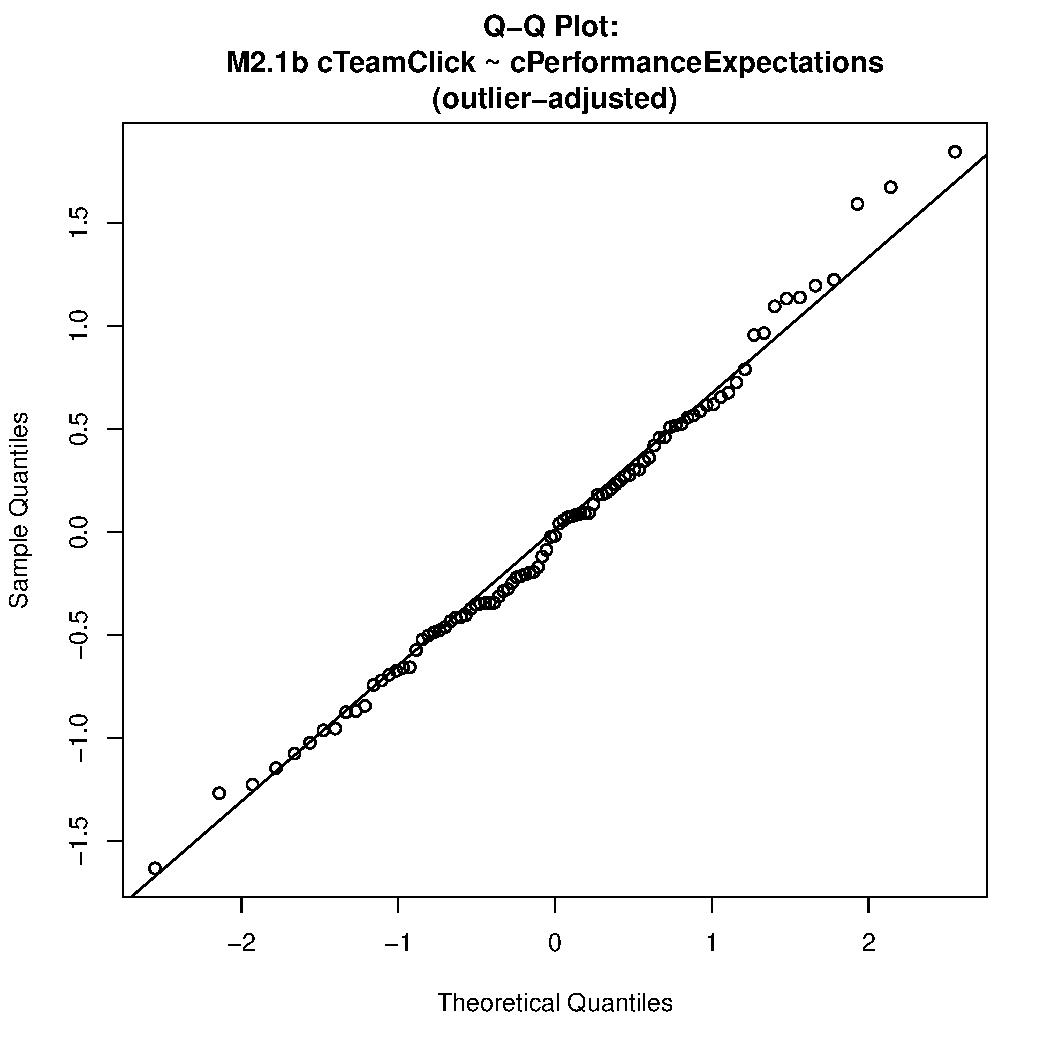
\includegraphics[scale =.4]{images/MLM21bOutQQNorm.pdf}
  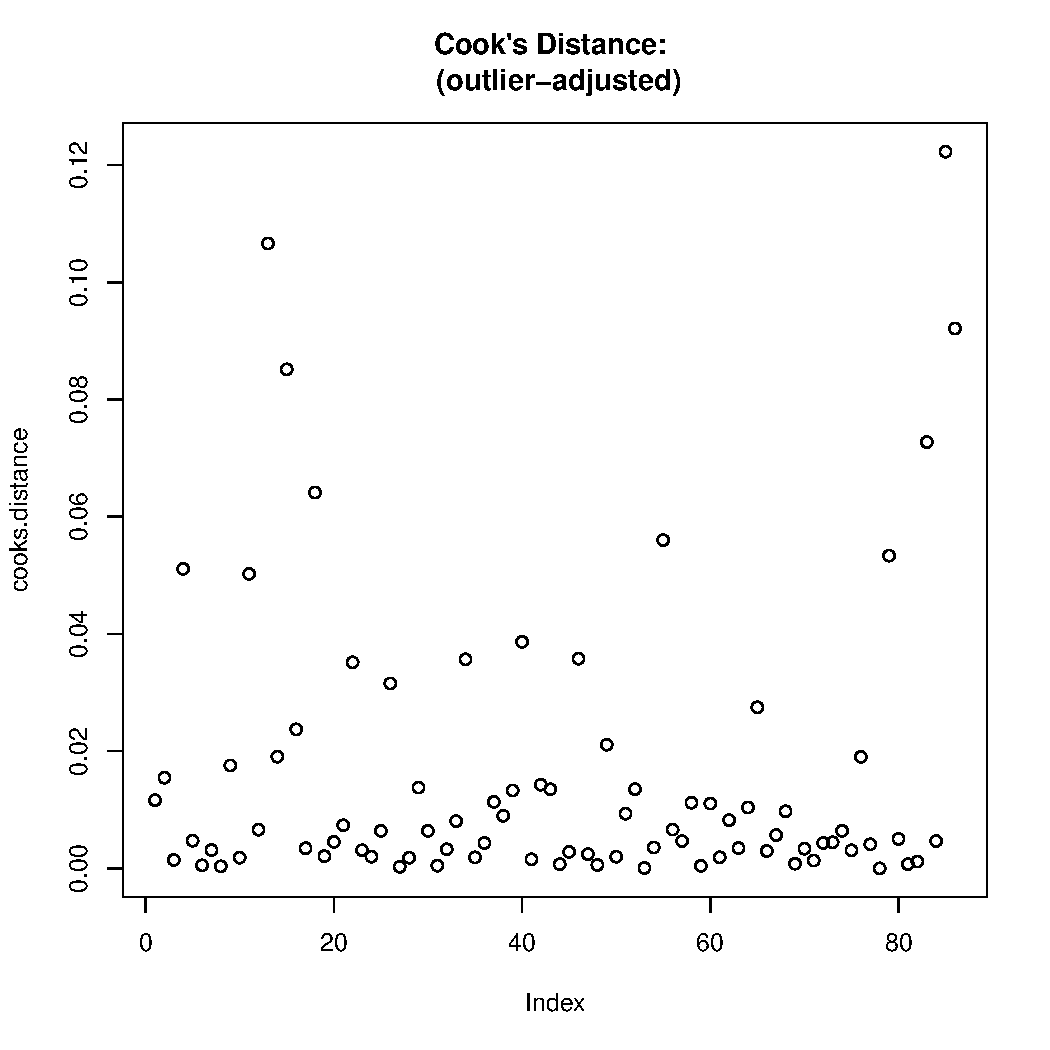
\includegraphics[scale =.4]{images/MLM21bOutCooksD.pdf}
  \caption{Model Assumptions: M2.1b Team Performance Expectations post-Tournament predicts change in Team Click (outliers removed)}
  \label{fig:MLM21bOutAssumptions}
\end{figure}



\begin{figure}[htbp]
  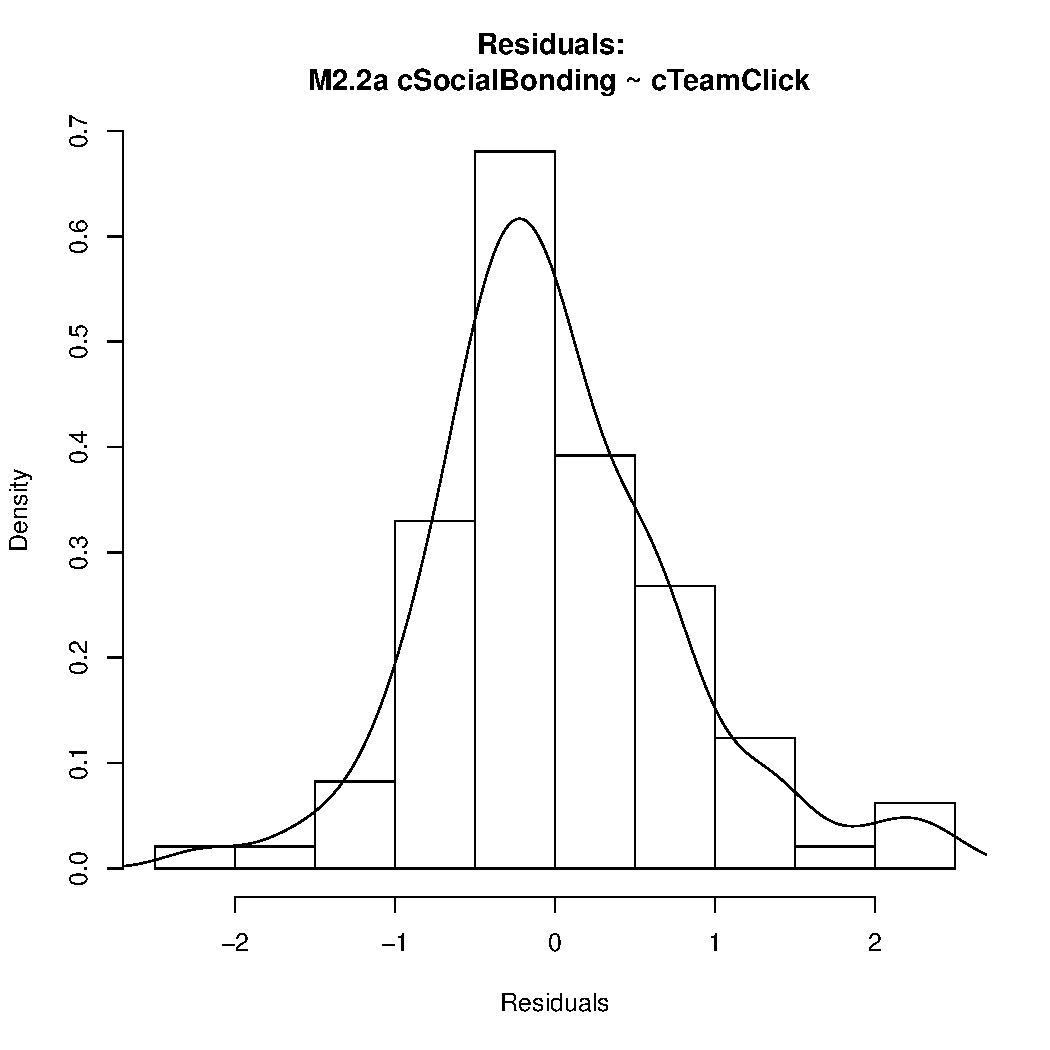
\includegraphics[scale =.4]{images/MLM22aHist.pdf}
  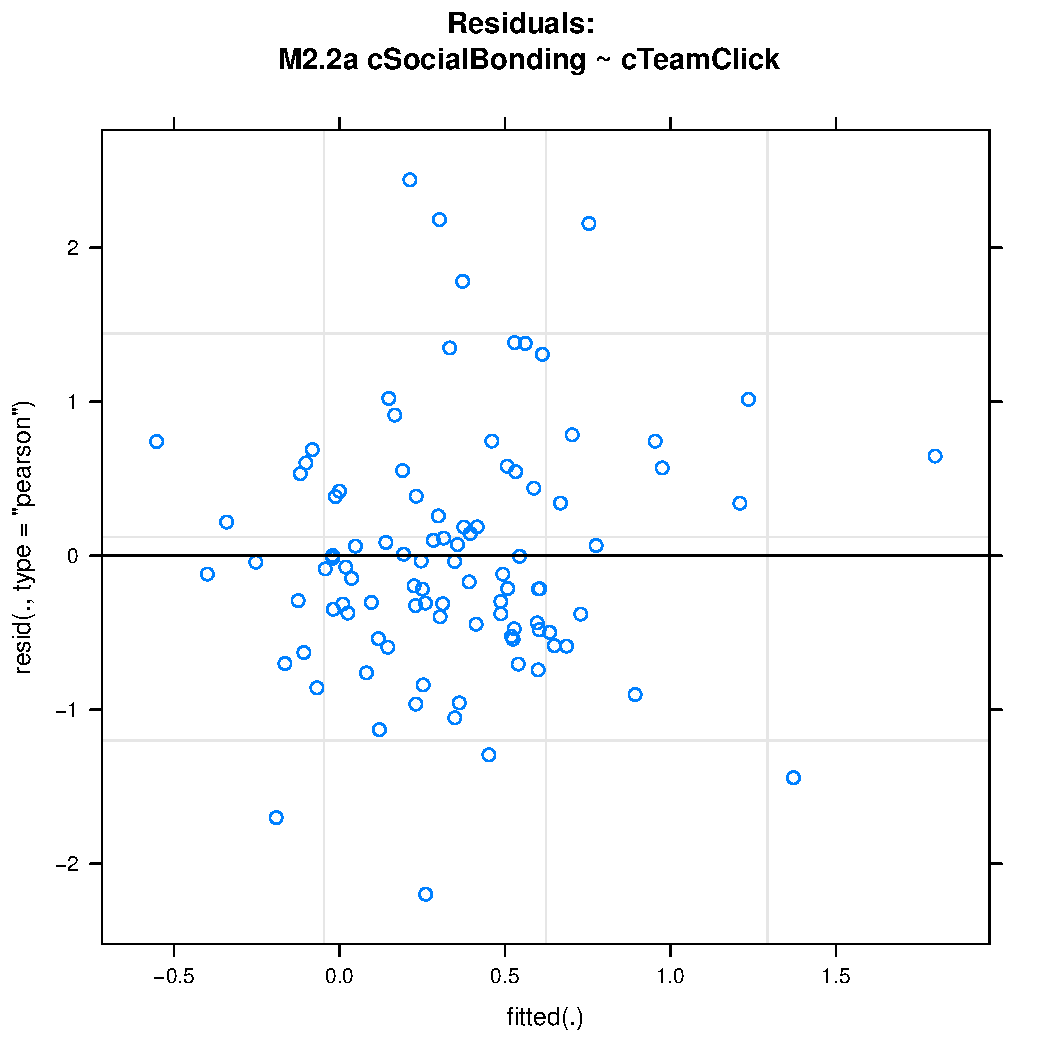
\includegraphics[scale =.4]{images/MLM22aScatter.pdf}
  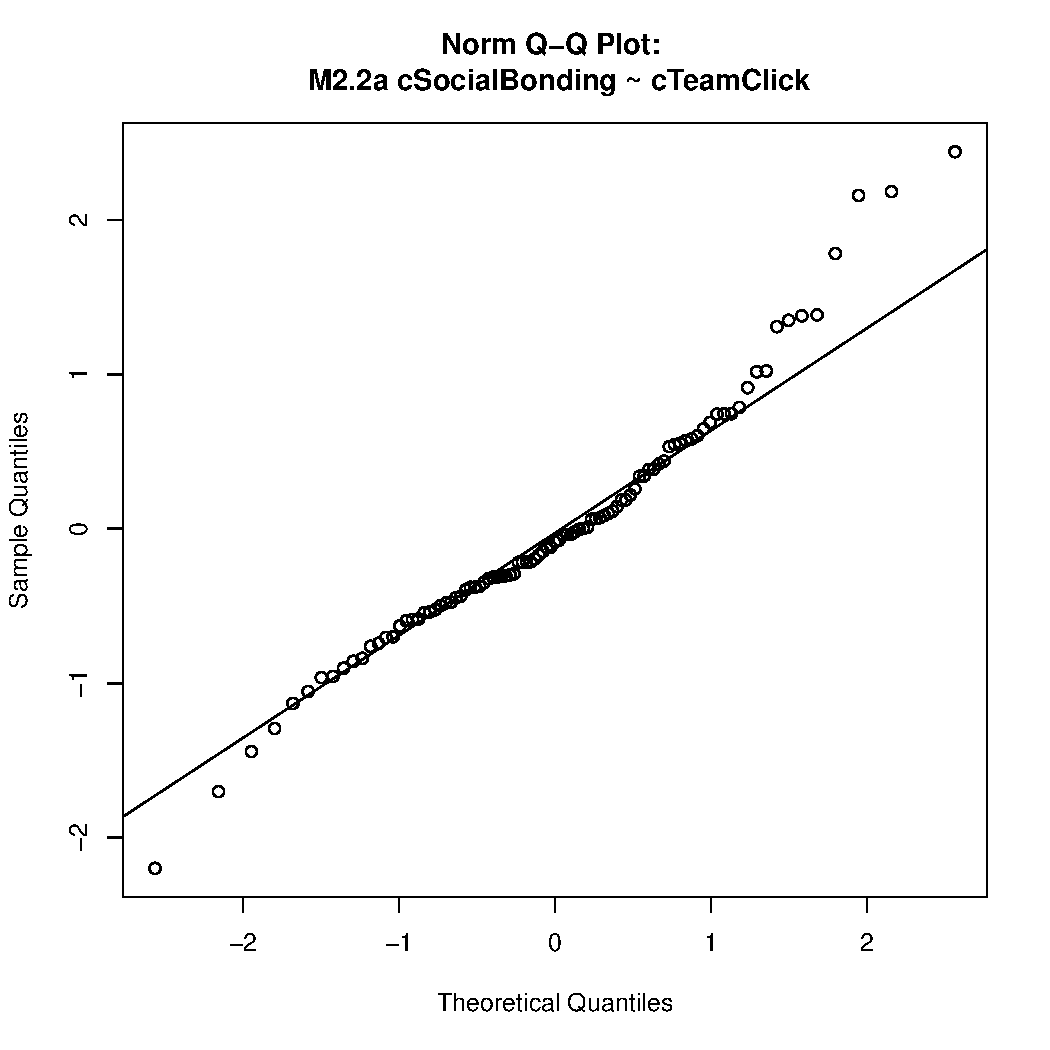
\includegraphics[scale =.4]{images/MLM22aQQNorm.pdf}
  \includegraphics[scale =.4]{images/MLM22aCooksD.pdf}
  \caption{Model Assumptions: M2.2a Change in Team Click predicts change in Social Bonding}
  \label{fig:MLM22aAssumptions}
\end{figure}


\begin{figure}[htbp]
  \includegraphics[scale =.4]{images/MLM23aHist.pdf}
  \includegraphics[scale =.4]{images/MLM23aScatter.pdf}
  \includegraphics[scale =.4]{images/MLM23aQQNorm.pdf}
  \includegraphics[scale =.4]{images/MLM23aCooksD.pdf}
  \caption{Model Assumptions: M2.3a Change in Joint Action Success predicts change in Social Bonding}
  \label{fig:MLM23aAssumptions}
\end{figure}



\begin{figure}[htbp]
  \includegraphics[scale =.4]{images/MLM23aHist.pdf}
  \includegraphics[scale =.4]{images/MLM23aScatter.pdf}
  \includegraphics[scale =.4]{images/MLM23aQQNorm.pdf}
  \includegraphics[scale =.4]{images/MLM23aCooksD.pdf}
  \caption{Model Assumptions: M2.3a Change in Joint Action Success predicts change in Social Bonding}
  \label{fig:MLM23aAssumptions}
\end{figure}
